\chapter{Uvod u programski jezik Pajton}

Pajton (\textit{Python}) je interpretirani, objektno-orijentisani programski jezik visokog nivoa opšte namjene. Razvio ga je holandski programer Guido van Rossum, a prva javna verzija jezika objavljena je u februaru 1991. godine. Naziv jezika potiče od britanske humorističke grupe \textit{Monty Python}, čiji je rad inspirisao autora tokom razvoja jezika.

Od svog nastanka Pajton je prošao kroz više razvojnih faza i danas predstavlja jedan od najrasprostranjenijih programskih jezika u akademskom i industrijskom okruženju. Njegova popularnost rezultat je prije svega jednostavne sintakse, velike čitljivosti koda i bogatog ekosistema biblioteka koje omogućavaju primjenu jezika u različitim oblastima. Pregled popularnosti programskih jezika prikazan je na Slici~\ref{fig: popular_program_lang}\footnote{Preuzeto sa {https://www.tiobe.com/tiobe-index/}}.

\begin{figure}[H]
	\centering
	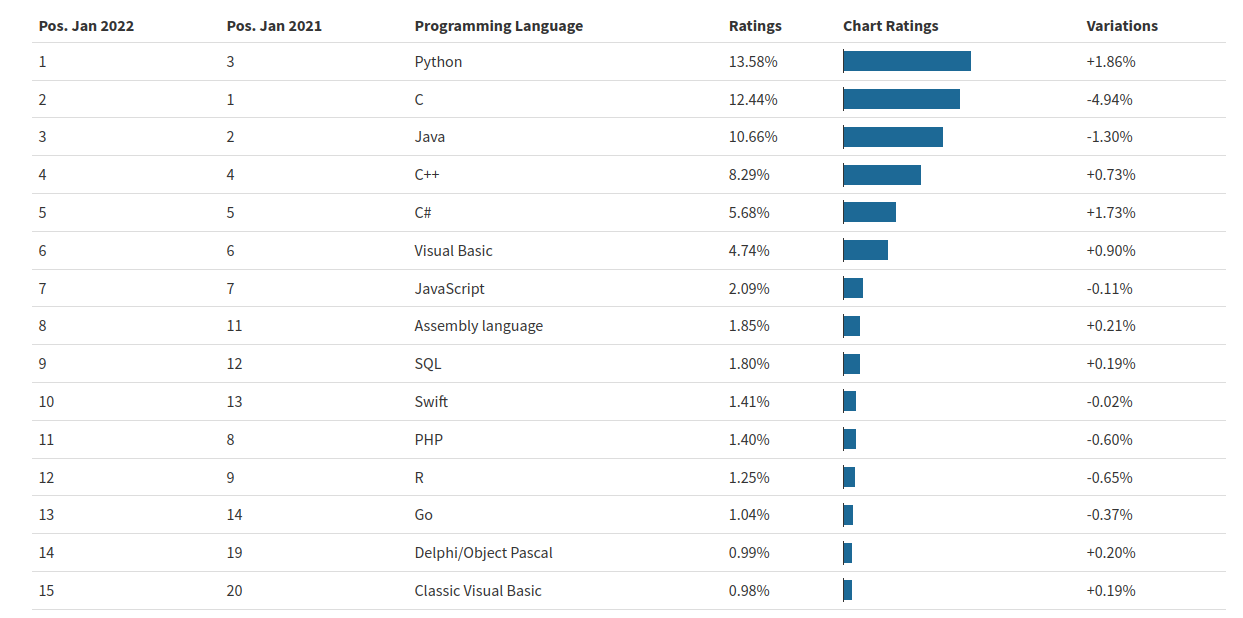
\includegraphics[width=400pt,height=190pt]{slike/most_popular_language.png}
	\caption{Statistički pregled najpopularnijih programskih jezika (2021--2022)}
	\label{fig: popular_program_lang}
\end{figure}

Početak razvoja Pajtona vezuje se za 1989. godinu, kada je Guido van Rossum započeo rad na novom programskom jeziku inspirisanom jezikom ABC. Cilj je bio kreiranje jezika koji bi zadržao jednostavnost i preglednost ABC-a, ali istovremeno pružio veću fleksibilnost i mogućnosti za razvoj složenijih softverskih sistema.

Prva verzija jezika, Pajton 0.9.0, objavljena je 1991. godine. Već tada su bili prisutni brojni koncepti koji i danas predstavljaju osnovu jezika, uključujući funkcije, klase, izuzetke i module.

Pajton 1.0 objavljen je 1994. godine i donio je dodatne funkcionalnosti inspirisane funkcionalnim programiranjem, kao što su funkcije \texttt{map}, \texttt{filter}, \texttt{reduce} i lambda izrazi. Verzija 2.0, objavljena 2000. godine, uvela je značajna unapređenja poput komprehenzije lista (\textit{list comprehensions}) i automatskog upravljanja memorijom putem sakupljača otpadaka (\textit{garbage collector}).

Velika prekretnica u razvoju jezika dogodila se 2008. godine objavljivanjem verzije Pajton 3.0. Ova verzija donijela je niz izmjena koje nisu bile u potpunosti kompatibilne sa prethodnim verzijama jezika, ali su omogućile jednostavniji, konzistentniji i pregledniji dizajn. Sve savremene verzije Pajtona zasnovane su na grani Pajton 3.

Danas se Pajton koristi u velikom broju oblasti, uključujući:

\begin{itemize}
	\item razvoj veb aplikacija;
	\item naučno i numeričko računarstvo;
	\item obradu i analizu podataka;
	\item mašinsko učenje i vještačku inteligenciju;
	\item automatizaciju zadataka i sistemsko programiranje;
	\item razvoj obrazovnog softvera.
\end{itemize}

Veliki doprinos popularnosti jezika daje i njegova izuzetno aktivna zajednica korisnika i programera. Tokom godina razvijen je veliki broj biblioteka i razvojnih okruženja koja značajno proširuju mogućnosti jezika. Među najpoznatijim bibliotekama nalaze se NumPy, Pandas, Matplotlib, SciPy, TensorFlow i PyTorch, dok su Django i Flask među najpopularnijim okvirima za razvoj veb aplikacija.

Pajton se posebno ističe jednostavnošću sintakse i čitljivošću programskog koda. Za razliku od mnogih drugih programskih jezika, naglasak je stavljen na preglednost i jasnoću programa, zbog čega se često preporučuje kao prvi programski jezik za učenje programiranja. Istovremeno, njegova izražajnost i bogat skup biblioteka čine ga pogodnim i za razvoj složenih profesionalnih softverskih sistema.

U ovoj knjizi Pajton će biti korišćen kao alat za implementaciju i eksperimentisanje sa različitim algoritamskim tehnikama. Njegova jednostavna sintaksa omogućava da se pažnja usmjeri na razumijevanje algoritama i struktura podataka, a ne na tehničke detalje implementacije karakteristične za jezike nižeg nivoa.\\

%ISHODI UCENJA:

Nakon uspješnog savladavanja sadržaja ove glave student će biti u stanju da:

\begin{itemize}
	\item objasni osnovne karakteristike programskog jezika Pajton i
	način predstavljanja podataka u memoriji;
	
	\item koristi osnovne numeričke i složene tipove podataka, uključujući
	stringove, liste, nizove, rječnike, skupove i torke;
	
	\item primijeni uslovne naredbe i petlje pri implementaciji
	jednostavnih proceduralnih algoritama;
	
	\item definiše i koristi funkcije, parametre, povratne vrijednosti i
	ugrađene funkcionalnosti za obradu kolekcija podataka;
	
	\item organizuje programski kod korištenjem modula i koristi odabrane
	module standardne biblioteke i eksternih biblioteka;
	
	\item prepoznaje, generiše i obrađuje izuzetke te koristi mehanizme za
	provjeru ispravnosti izvršavanja programa;
	
	\item koristi datoteke,  regularne izraze za učitavanje,
	obradu i zapisivanje strukturiranih podataka;
	
	\item objasni osnovne faze izvršavanja Pajton programa, uključujući
	generisanje bajtkoda, ulogu virtuelne mašine i osnovne principe
	upravljanja memorijom.
\end{itemize}

\section{Osnovne karakteristike}

Pajton posjeduje niz osobina koje ga čine pogodnim kako za učenje programiranja, tako i za razvoj složenih softverskih sistema. U nastavku navodimo njegove najvažnije karakteristike.

\begin{itemize}
	\item \textit{Jezik visokog nivoa} (\textit{high-level language}). Pajton omogućava programiranje na visokom nivou apstrakcije, pri čemu se programer može fokusirati na rješavanje problema, a ne na detalje rada računara. Sintaksa jezika je jednostavna i pregledna, zbog čega je k\^od relativno lako čitati i održavati.
	
	\item \textit{Dinamički tipiziran jezik}. Tip promjenljive određuje se tokom izvršavanja programa. Zbog toga nije potrebno unaprijed deklarisati tip svake promjenljive. Na primjer, ista promjenljiva može u jednom trenutku sadržavati cijeli broj, a kasnije tekstualnu vrijednost.
	
	\item \textit{Objektno-orijentisani jezik}. U Pajtonu su podaci i operacije nad njima organizovani kroz objekte i klase. Objektno-orijentisano programiranje omogućava modelovanje problema pomoću objekata i njihovih međusobnih interakcija, što često dovodi do preglednijeg i modularnijeg koda.
	
	\item \textit{Interpretirani i skriptni jezik}. Programi napisani u Pajtonu izvršavaju se posredstvom interpretera, bez potrebe za klasičnim procesom kompajliranja kakav postoji kod jezika poput C ili C++. Zbog toga je razvoj programa brz i pogodan za automatizaciju različitih zadataka.
	
	\item \textit{Automatsko upravljanje memorijom}. Pajton posjeduje ugrađene mehanizme za automatsko oslobađanje memorije koja više nije potrebna programu (\textit{garbage collection}). Time se značajno smanjuje mogućnost grešaka povezanih sa ručnim upravljanjem memorijom.

\end{itemize}

Zahvaljujući ovim karakteristikama, Pajton se danas koristi u obrazovanju, naučnim istraživanjima, analizi podataka, vještačkoj inteligenciji, razvoju veb aplikacija i mnogim drugim oblastima.

\section{Pregled ugrađenih tipova podataka}

Pajton posjeduje veliki broj ugrađenih (\textit{built-in}) tipova podataka koji su dostupni bez potrebe za instalacijom dodatnih biblioteka. Svaki tip podataka definiše način predstavljanja i manipulacije određenom vrstom informacija.

Najvažniji ugrađeni tipovi podataka su:

\begin{itemize}
	\item numerički tipovi: \texttt{int}, \texttt{float}, \texttt{complex};
	
	```
	\item tekstualni tipovi: \texttt{str};
	
	\item sekvencijalni tipovi: \texttt{list}, \texttt{tuple}, \texttt{range};
	
	\item mapirajući tipovi: \texttt{dict};
	
	\item skupovni tipovi: \texttt{set}, \texttt{frozenset};
	
	\item logički tip: \texttt{bool};
	
	\item binarni tipovi: \texttt{bytes}, \texttt{bytearray}, \texttt{memoryview}.
	```
	
\end{itemize}

Ovi tipovi predstavljaju osnovu za izgradnju složenijih struktura podataka i implementaciju različitih algoritama. U nastavku poglavlja detaljno ćemo razmotriti najvažnije od njih.

\section{Deklarisanje varijabli i memorijska organizacija}

Promjenljive u Pajtonu kreiraju se dodjelom vrijednosti pomoću operatora dodjele \texttt{=}.

Za razliku od mnogih drugih programskih jezika, nije potrebno unaprijed deklarisati tip promjenljive. Pajton automatski određuje odgovarajući tip na osnovu dodijeljene vrijednosti.

Na primjer, promjenljiva \texttt{x} kojoj se dodjeljuje cijeli broj 5 kreira se na sljedeći način:

\begin{minted}{python}
	x = 5
\end{minted}

Slično tome, promjenljivoj \texttt{y} možemo dodijeliti tekstualnu vrijednost:

\begin{minted}{python}
	y = "abc"
\end{minted}

Prilikom izvršavanja programa Pajton kreira odgovarajuće objekte u memoriji, dok promjenljive predstavljaju reference na te objekte. Zbog toga promjenljiva ne sadrži nužno samu vrijednost, već informaciju o tome gdje se odgovarajući objekat nalazi u memoriji.

U narednim sekcijama detaljnije ćemo razmotriti numeričke, tekstualne i složene tipove podataka, kao i način njihovog korištenja u programima.

 Pajton je objektno-orijentisani programski jezik, što znači da se sve vrijednosti u programu predstavljaju kao objekti. Drugim riječima, svaka promjenljiva zapravo referencira neki objekat smješten u memoriji.
 
 Na primjer, promjenljiva koja sadrži cijeli broj predstavlja referencu na objekat tipa \texttt{int}, dok promjenljiva koja sadrži tekst predstavlja referencu na objekat tipa \texttt{str}. U tom smislu, promjenljive u Pajtonu ne čuvaju direktno vrijednosti, već reference na objekte koji sadrže te vrijednosti.
 
 Posmatrajmo sljedeći primjer:
 
 \begin{minted}{python}
 	x = 42
 \end{minted}
 
 Promjenljiva \texttt{x} referencira objekat koji predstavlja broj 42, što se može ilustrovati kao na Slici~\ref{fig:var_object}.
 
 \begin{figure}[H]
 	\centering
 	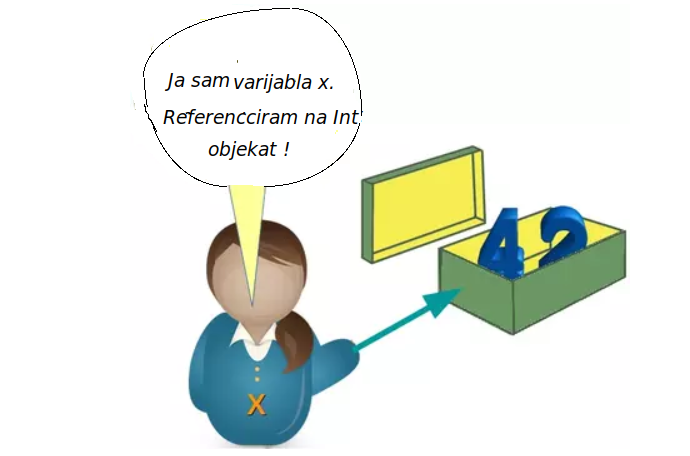
\includegraphics[width=140pt,height=100pt]{slike/variable_object.png}
 	\caption{Promjenljiva \texttt{x} referencira objekat vrijednosti 42.}
 	\label{fig:var_object}
 \end{figure}
 
 Ako zatim napišemo
 
 \begin{minted}{python}
 	y = x
 \end{minted}
 
 promjenljiva \texttt{y} neće dobiti kopiju broja 42, već će referencirati isti objekat kao i promjenljiva \texttt{x}. Situacija je prikazana na Slici~\ref{fig:two_refs}.
 
 \begin{figure}[H]
 	\centering
 	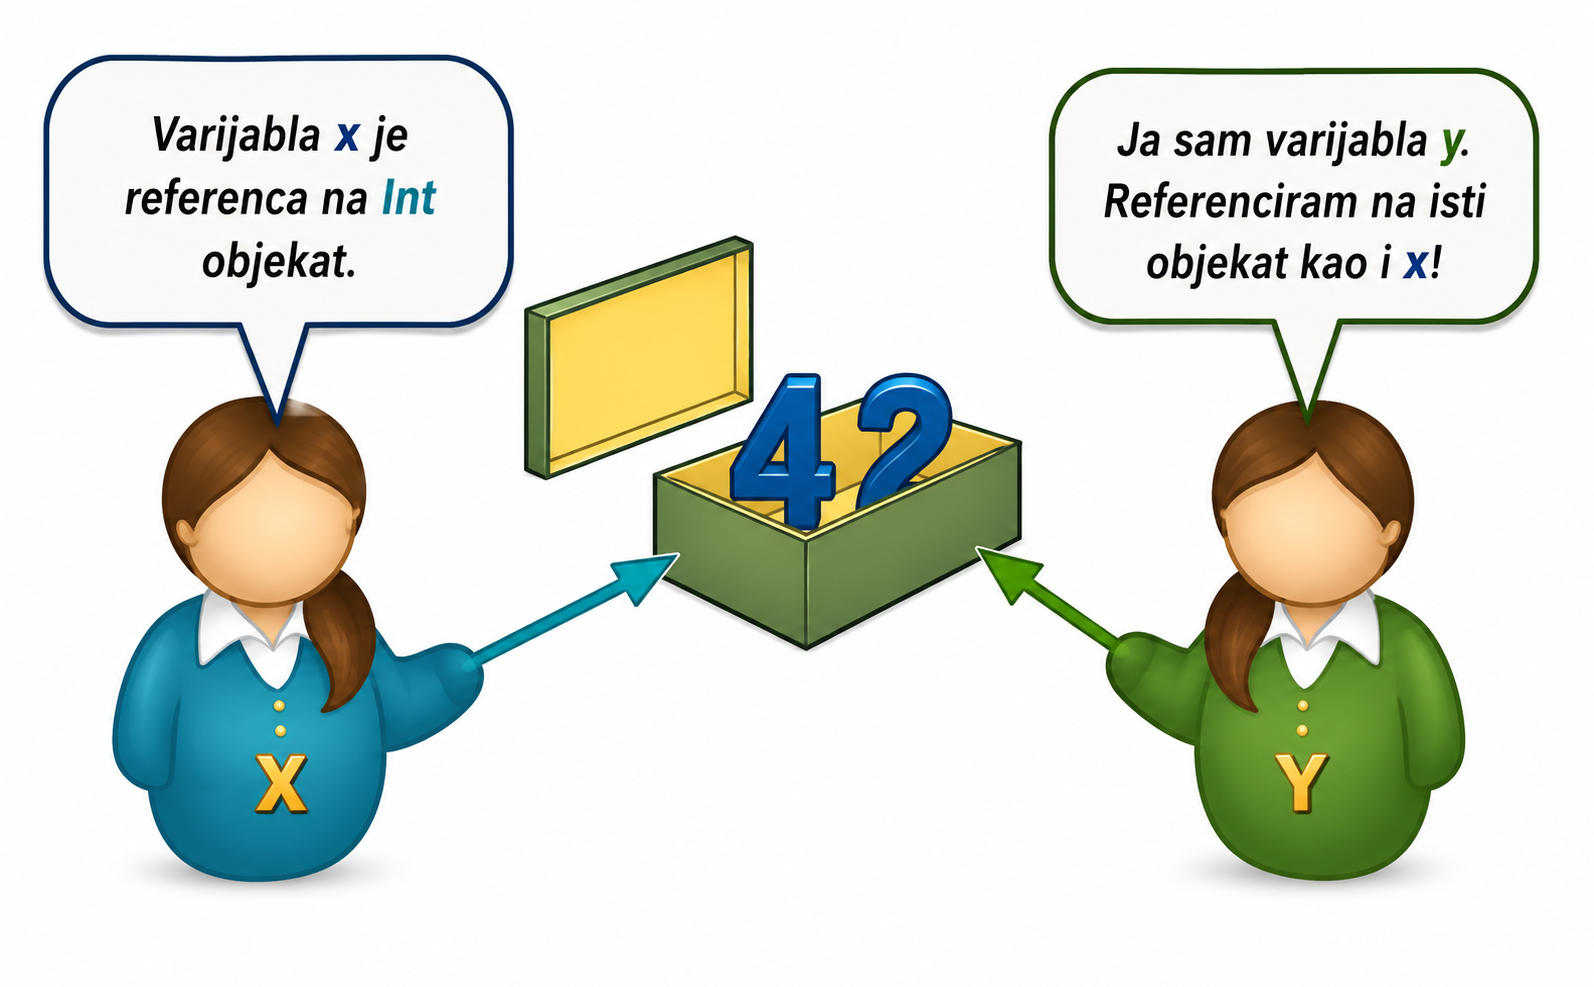
\includegraphics[width=140pt,height=100pt]{slike/point_two_vars.png}
 	\caption{Dvije promjenljive referenciraju isti objekat.}
 	\label{fig:two_refs}
 \end{figure}
 
 Ukoliko nakon toga izvršimo naredbu
 
 \begin{minted}{python}
 	y = 72
 \end{minted}
 
 promjenljiva \texttt{y} počinje referencirati novi objekat, dok \texttt{x} i dalje pokazuje na objekat koji predstavlja broj 42.
 
 \begin{figure}[H]
 	\centering
 	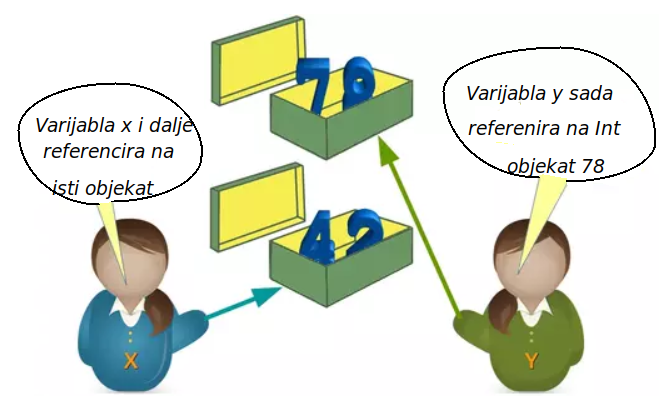
\includegraphics[width=140pt,height=100pt]{slike/vars_different_assigned.png}
 	\caption{Promjenljive referenciraju različite objekte.}
 \end{figure}
 
 Slično tome, promjenljivoj možemo dodijeliti objekat potpuno drugog tipa:
 
 \begin{minted}{python}
 	x = "Text"
 \end{minted}
 
 Nakon izvršavanja ove naredbe promjenljiva \texttt{x} više ne referencira objekat tipa \texttt{int}, već objekat tipa \texttt{str}.
 
 \begin{figure}[H]
 	\centering
 	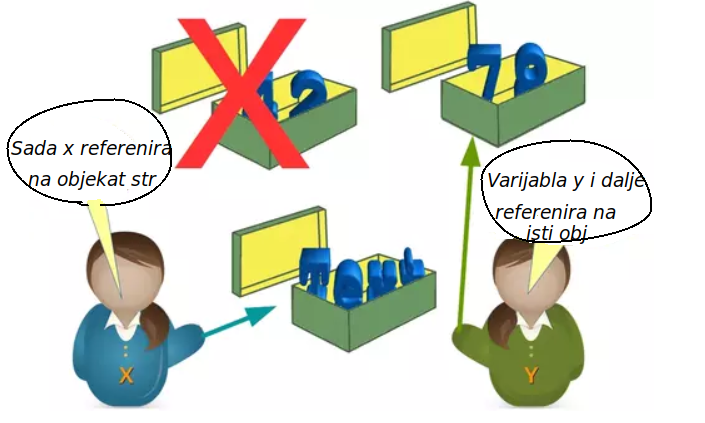
\includegraphics[width=140pt,height=100pt]{slike/varX_different_assigned.png}
 	\caption{Promjena reference promjenljive \texttt{x}.}
 \end{figure}
 
 Ovakvo ponašanje posljedica je činjenice da je Pajton dinamički tipiziran jezik. Tip se vezuje za objekat, a ne za promjenljivu. Zbog toga ista promjenljiva tokom izvršavanja programa može referencirati objekte različitih tipova.
 
 Ipak, od verzije Pajton 3.5 moguće je koristiti oznake tipova (\textit{type hints}) radi bolje čitljivosti programa:
 
 \begin{minted}{python}
 	x: str = "abc"
 	y: int = 23
 \end{minted}
 
 Napomenimo da ove oznake ne mijenjaju način rada jezika, već prvenstveno služe kao dokumentacija i pomoć alatima za statičku analizu koda.
 
 \subsection*{Upravljanje memorijom}
 
 Pajton automatski upravlja memorijom. Svaki objekat posjeduje brojač referenci koji prati koliko promjenljivih ili drugih objekata trenutno pokazuje na njega.
 
 Kada broj referenci nekog objekta postane jednak nuli, objekat više nije dostupan programu i njegova memorija može biti oslobođena. Pored toga, Pajton koristi i mehanizam sakupljanja otpadaka (\textit{garbage collection}) koji uklanja objekte koji više nisu potrebni, uključujući i složenije slučajeve kružnih referenci.
 
 Zahvaljujući ovim mehanizmima, programer uglavnom ne mora ručno voditi računa o dodjeljivanju i oslobađanju memorije, što značajno pojednostavljuje razvoj programa.
 
 Adresu objekta na koji referencira promjenljiva moguće je dobiti pomoću funkcije \texttt{id()}:
 
 \begin{minted}{python}
 	idnum = id(x)
 	idhex = hex(id(x))
 \end{minted}
 
 Dobijena vrijednost predstavlja jedinstveni identifikator objekta tokom njegovog životnog vijeka.
 
 \subsection*{Ispis i komentari}
 
 Ispis rezultata na ekran vrši se pomoću funkcije \texttt{print()}:
 
 \begin{minted}{python}
 	print("Pozdrav svijete!")
 	print(x)
 \end{minted}
 
 Funkcija \texttt{print()} može prikazati tekst, brojeve i druge objekte. Prije ispisa, objekat se po potrebi pretvara u tekstualni oblik.
 
 Komentari služe za dokumentovanje programa i ne izvršavaju se tokom rada programa.
 
 Jednolinijski komentar započinje znakom {\#}:
 
 \begin{minted}{python}
 	
 	# Ovo je komentar
 	
 	x = 5
 \end{minted}
 
 Za višelinijske komentare ili dokumentacione stringove najčešće se koriste trostruki navodnici:
 
 \begin{minted}{python}
 	"""
 	Ovo je višelinijski komentar
 	ili dokumentacioni string.
 	"""
 \end{minted}
 
 Komentari povećavaju čitljivost programa i olakšavaju njegovo održavanje, naročito kod većih projekata.
 

\section{Osnovni numerički tipovi podataka}

Numerički tipovi podataka koriste se za predstavljanje brojeva i izvođenje aritmetičkih operacija nad njima. Pajton podržava nekoliko numeričkih tipova, od kojih su najvažniji \texttt{int}, \texttt{float} i \texttt{complex}.

\subsection{Cjelobrojni i realni brojevi}

Tip \texttt{int} (skraćeno od \textit{integer}) koristi se za predstavljanje cijelih brojeva, dok tip \texttt{float} (skraćeno od \textit{floating-point number}) služi za predstavljanje realnih brojeva.

Primjeri inicijalizacije ovih tipova dati su u nastavku:

\begin{minted}{python}
	x = 5         # int
	y = -3        # int
	
	z = 3.14      # float
	w = -0.325    # float
\end{minted}

Nad numeričkim tipovima moguće je primjenjivati standardne aritmetičke operacije kao što su sabiranje (\texttt{+}), oduzimanje (\texttt{-}), množenje (\texttt{*}) i dijeljenje (\texttt{/}).

Posebnu pažnju treba obratiti na operatore dijeljenja:

\begin{itemize}
	\item \texttt{/} -- realno dijeljenje;
	\item \texttt{//} -- cjelobrojno dijeljenje.
\end{itemize}

Na primjer:

\begin{minted}{python}
	print(5 / 2)   # 2.5
	print(5 // 2)  # 2
\end{minted}

Pored osnovnih operatora, Pajton pruža i veliki broj ugrađenih funkcija za rad sa brojevima. Neke od najčešće korištenih su:

\begin{itemize}
	\item \texttt{abs(x)} -- apsolutna vrijednost broja;
	\item \texttt{round(x)} -- zaokruživanje broja;
	\item \texttt{min(...)} -- najmanja vrijednost;
	\item \texttt{max(...)} -- najveća vrijednost.
\end{itemize}

\begin{example}
	\begin{minted}{python}
		print(abs(-7))          # 7
		print(round(3.14159,2)) # 3.14
		print(min(2, 5, -1))    # -1
		print(max(2, 5, -1))    # 5
	\end{minted}
\end{example}

\subsection{Kompleksni brojevi}

Tip \texttt{complex} koristi se za predstavljanje kompleksnih brojeva oblika

$
a+bj,
$

gdje su $a$ i $b$ realni brojevi, dok simbol \texttt{j} predstavlja imaginarnu jedinicu.

Primjer rada sa kompleksnim brojevima:

\begin{minted}{python}
	x = 1 + 1j
	y = 2 + 1j
	
	z = x + y
	
	print(z)       # (3+2j)
	print(z.real)  # 3.0
	print(z.imag)  # 2.0
\end{minted}

Realni i imaginarni dio kompleksnog broja mogu se dobiti pomoću atributa \texttt{real} i \texttt{imag}.

Kompleksni broj moguće je kreirati i korišćenjem funkcije \texttt{complex()}:

\begin{minted}{python}
	z = complex(3, 2)
	print(z)   # (3+2j)
\end{minted}

Prvi argument predstavlja realni dio, dok drugi argument predstavlja imaginarni dio kompleksnog broja.

\section{Naredbe grananja i petlje}

U ovoj sekciji upoznaćemo osnovne kontrolne strukture programskog jezika Pajton: naredbu grananja \texttt{if} te petlje \texttt{for} i \texttt{while}.

Prije toga, u Tabeli~\ref{fig: operatori_poredjenja} dati su najčešće korišteni operatori poređenja.

Svaki izraz poređenja vraća logičku vrijednost \texttt{True} ili \texttt{False}, u zavisnosti od toga da li je odgovarajući uslov ispunjen.

\begin{table}[H]
	\caption{Osnovni operatori poređenja u Pajtonu.}
	\label{fig: operatori_poredjenja}
	
	\centering
	\scalebox{0.85}{
	\begin{tabular}{lll}
		\textbf{Matematička notacija} &
		\textbf{Pajtonova notacija} &
		\textbf{Značenje} \\ \hline
		
		$a < b$ & \texttt{a < b} &
		$a$ je manje od $b$ \\
		
		$a \leq b$ & \texttt{a <= b} &
		$a$ je manje ili jednako od $b$ \\
		
		$a > b$ & \texttt{a > b} &
		$a$ je veće od $b$ \\
		
		$a \geq b$ & \texttt{a >= b} &
		$a$ je veće ili jednako od $b$ \\
		
		$a = b$ & \texttt{a == b} &
		$a$ je jednako $b$ \\
		
		$a \neq b$ & \texttt{a != b} &
		$a$ nije jednako $b$ \\ \hline
	\end{tabular}}
	
\end{table}

\subsection{Uslovna naredba \texttt{if}}

Najjednostavniji oblik naredbe grananja dat je sljedećom sintaksom:

\begin{minted}{python}
	if uslov:
	    naredba_1
	else:
	    naredba_2
\end{minted}

Tok izvršavanja je jednostavan:

\begin{itemize}
	\item ako je uslov tačan, izvršava se blok \texttt{naredba\_1};
	\item u suprotnom se izvršava blok \texttt{naredba\_2}.
\end{itemize}

Posebno treba obratiti pažnju na uvlačenje koda (\textit{indentation}). Za razliku od mnogih drugih programskih jezika, u Pajtonu uvlačenje nije samo pitanje stila, već predstavlja dio sintakse jezika.

Nakon izvršavanja odgovarajućeg bloka program nastavlja sa prvom naredbom koja se nalazi izvan \texttt{if}-strukture.

U situacijama kada postoji više alternativa koristi se naredba \texttt{elif}:

\begin{minted}{python}
	if uslov_1:
	    naredba_1
	elif uslov_2:
	    naredba_2
	elif uslov_3:
	    naredba_3
	else:
	    naredba_n
\end{minted}

Uslovi se provjeravaju redom, od vrha prema dnu. Čim se pronađe prvi tačan uslov, izvršava se odgovarajući blok naredbi, nakon čega se ostatak strukture preskače.

Ako nijedan od uslova nije zadovoljen, izvršava se blok pod granom \texttt{else}.

\subsection{For i While petlje}

Petlje predstavljaju kontrolne strukture koje omogućavaju višestruko izvršavanje istog bloka koda. Koriste se kada je potrebno ponoviti određene operacije unaprijed poznat broj puta ili sve dok je zadovoljen određeni uslov.

Pajton podržava dvije osnovne vrste petlji:

\begin{itemize}
	\item \texttt{for} petlju;
	\item \texttt{while} petlju.
\end{itemize}

\subsubsection*{\texttt{for} petlja}

\texttt{for} petlja koristi se za prolazak kroz elemente iterabilnih objekata, kao što su liste, torke, stringovi, skupovi i rječnici.

Njena osnovna sintaksa je:

\begin{minted}{python}
	for item in iterable:
	    naredba
\end{minted}

Promjenljivoj \texttt{item} redom se dodjeljuju elementi kolekcije \texttt{iterable}, a za svaki element izvršava se odgovarajući blok koda.

Na primjer:

\begin{minted}{python}
	for broj in [1, 2, 3, 4]:
	    print(broj)
\end{minted}

Izvršavanjem ovog programa na ekran će biti ispisani brojevi 1, 2, 3 i 4.

Vrlo često se \texttt{for} petlja koristi zajedno sa funkcijom \texttt{range()}:

\begin{minted}{python}
	for i in range(5):
	    print(i)
\end{minted}

Ovaj kod ispisuje brojeve od 0 do 4.

\subsubsection*{\texttt{while} petlja}

\texttt{while} petlja izvršava blok koda sve dok je zadovoljen zadati logički uslov.

Njena osnovna sintaksa je:

\begin{minted}{python}
	while uslov:
	    naredba
\end{minted}

Prije svake iteracije provjerava se vrijednost izraza \texttt{uslov}. Ako je njegova vrijednost \texttt{True}, izvršava se tijelo petlje. Kada uslov postane netačan (\texttt{False}), izvršavanje petlje se završava, a program nastavlja sa prvom naredbom nakon petlje.

Na primjer, prvih deset parnih prirodnih brojeva može se ispisati na sljedeći način:

\begin{minted}{python}
	i = 1
	
	while i <= 10:
	    print(2 * i)
	    i += 1
\end{minted}

Naredba
\begin{minted}{python}
	i += 1
\end{minted}
predstavlja skraćeni zapis za

\begin{minted}{python}
	i = i + 1
\end{minted}

i koristi se za povećavanje vrijednosti promjenljive za jedan.

\section{Složene strukture podataka}

Pored osnovnih numeričkih tipova podataka, Pajton pruža i niz složenijih struktura podataka koje omogućavaju efikasno organizovanje i obradu većih količina informacija.

Najvažnije među njima su:

\begin{itemize}
	\item stringovi (\texttt{str});
	\item liste (\texttt{list});
	\item torke (\texttt{tuple});
	\item skupovi (\texttt{set});
	\item rječnici (\texttt{dict}).
\end{itemize}

Sve navedene strukture predstavljaju kolekcije objekata i koriste se u gotovo svakom ozbiljnijem programu.

\subsection{Stringovni tip podataka}

Tip \texttt{str} predstavlja ugrađeni tip podataka namijenjen radu sa tekstom. String se može posmatrati kao uređena sekvenca Unicode znakova.

Jedna od najvažnijih osobina stringova jeste da su \textit{nepromjenjivi} (\textit{immutable}). Nakon što se string kreira, njegov sadržaj nije moguće direktno mijenjati. Svaka izmjena zapravo rezultuje kreiranjem novog string objekta.

\subsubsection*{Inicijalizacija stringova}

String se može definisati korišćenjem jednostrukih ili dvostrukih navodnika:

\begin{minted}{python}
	string0 = 'hello'
	string1 = "world"
\end{minted}

Za višelinijske stringove koriste se trostruki navodnici:

\begin{minted}{python}
	multiline_str = """
	Ovo je
	višelinijski string.
	"""
\end{minted}

\subsubsection*{Osnovne operacije nad stringovima}

\begin{itemize}
	
	\item \textbf{Konkatenacija}
	
	Stringovi se mogu spajati pomoću operatora \texttt{+}:
	
	\begin{minted}{python}
		ime = "Marko"
		prezime = "Markovic"
		
		print(ime + " " + prezime)
	\end{minted}
	

	\item \textbf{Pristup pojedinačnim znakovima}
	
	Znakovima stringa pristupa se pomoću operatora indeksiranja \texttt{[]}.
	```
	
	\begin{minted}{python}
		tekst = "Python"
		
		print(tekst[0])   # P
		print(tekst[-1])  # n
	\end{minted}
	
	Pozitivni indeksi broje se od početka stringa, dok negativni indeksi broje od kraja stringa.
	
	\item \textbf{Rezanje stringa (slicing)}
	
	Dio stringa može se izdvojiti pomoću operatora \texttt{[:]}:
	
	\begin{minted}{python}
		tekst = "world"
		
		print(tekst[1:3])  # or
		print(tekst[:3])   # wor
		print(tekst[2:])   # rld
	\end{minted}
	
	\item \textbf{Ponavljanje stringa}
	
	Operator \texttt{*} omogućava višestruko ponavljanje stringa:
	
	\begin{minted}{python}
		print("abc" * 3)
	\end{minted}
	
	Rezultat je:
	
	\begin{minted}{text}
		abcabcabc
	\end{minted}
	\item \textbf{Dužina stringa}
	
	Broj znakova u stringu dobija se funkcijom \texttt{len()}:
	
	\begin{minted}{python}
		print(len("Python"))
	\end{minted}
	
	\item \textbf{Brisanje reference}
	
	Ključna riječ \texttt{del} uklanja referencu na objekat:
	
	\begin{minted}{python}
		tekst = "abc"
		del tekst
	\end{minted}
	
\end{itemize}

\subsubsection*{Korisne metode}

Klasa \texttt{str} sadrži veliki broj ugrađenih metoda. Neke od najčešće korištenih su:

\begin{itemize}
	\item \texttt{lower()} -- pretvara sva slova u mala;
	\item \texttt{upper()} -- pretvara sva slova u velika;
	\item \texttt{strip()} -- uklanja praznine sa početka i kraja stringa;
	\item \texttt{replace()} -- zamjenjuje dio stringa drugim tekstom;
	\item \texttt{find()} -- pronalazi poziciju podstringa.
\end{itemize}

Njihovu detaljniju upotrebu prikazaćemo kroz naredne primjere.

\textit{Memorijska organizacija}. Stringovi se u Pajtonu predstavljaju kao uređene sekvence Unicode znakova smještene u neprekidnom dijelu memorije. Svakom znaku pridružen je odgovarajući Unicode k\^od, što omogućava rad sa tekstom na velikom broju svjetskih jezika.

Pojednostavljen prikaz memorijske organizacije stringa

\begin{minted}{python}
	x = "code"
\end{minted}

dat je na Slici~\ref{fig:str_mem}.

\begin{figure}[H]
	\centering
	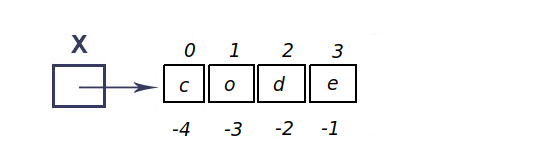
\includegraphics[width=200pt,height=60pt]{slike/str_mem_organization.png}
	\caption{Pojednostavljen prikaz memorijske organizacije stringa \texttt{"code"}.}
	\label{fig:str_mem}
\end{figure}

Za razliku od nekih drugih programskih jezika, stringovi u Pajtonu su \textit{nepromjenjivi} (\textit{immutable}). To znači da se sadržaj postojećeg stringa ne može direktno mijenjati. Svaka operacija koja naizgled mijenja string zapravo kreira novi string objekat.

Na primjer:

\begin{minted}{python}
	s = "code"
	s = s + "!"
\end{minted}

Nakon izvršavanja druge naredbe kreira se novi string \texttt{"code!"}, dok originalni string ostaje nepromijenjen.

\textit{Dodatna napomena}. Pajton interno koristi različite optimizacije za rad sa stringovima. Jedna od njih je \textit{interniranje stringova} (\textit{string interning}), pri čemu se identični stringovi po potrebi mogu dijeliti između više promjenljivih. Time se smanjuje potrošnja memorije i poboljšavaju performanse programa.

\subsubsection*{Formatiranje stringova}

Prilikom ispisa rezultata često je potrebno kombinovati tekst i vrijednosti promjenljivih. Pajton nudi nekoliko načina za formatiranje stringova.

Jedan od tradicionalnih pristupa koristi metodu \texttt{format()}:

\begin{minted}{python}
	print("Moje ime je {0}, a prezime {1}".
	       format("Marko", "Marković"))
\end{minted}

Vrijednost označena sa \texttt{{0}} zamjenjuje se prvim argumentom funkcije \texttt{format()}, dok se \texttt{{1}} zamjenjuje drugim argumentom.

Savremeniji i danas preporučeni način predstavljaju formatirani stringovi (\textit{f-strings}):

\begin{minted}{python}
	ime = "Marko"
	godine = 32
	print(f"Ime: {ime}, godine: {godine}")
\end{minted}

Kod f-stringova vrijednosti promjenljivih navode se direktno unutar vitičastih zagrada, što k\^od čini preglednijim i jednostavnijim za pisanje.

Zbog svoje čitljivosti i efikasnosti, f-stringovi predstavljaju preporučeni način formatiranja stringova u savremenom Pajtonu.


\subsection{Liste}

Lista predstavlja uređenu, indeksiranu i promjenljivu kolekciju elemenata. U Pajtonu se implementira pomoću ugrađenog tipa podataka \texttt{list}.

Za razliku od mnogih drugih programskih jezika, elementi liste ne moraju biti istog tipa. Zbog toga kažemo da su liste \textit{heterogene} kolekcije. Na primjer, ista lista može sadržavati brojeve, stringove, logičke vrijednosti i druge objekte.

Elementi liste indeksiraju se brojevima počevši od nule. Pored standardnog indeksiranja, Pajton podržava i negativne indekse. Pri tome indeks \texttt{-1} označava posljednji element liste, \texttt{-2} pretposljednji itd.

\subsubsection*{Inicijalizacija lista}

Liste se mogu kreirati na više načina:

\begin{minted}{python}
	lista = list()
	lista1 = ["a", "b", 2.0, 3]	
	lista2 = list(("abc", "def", 2))
\end{minted}

\subsubsection*{Pristup elementima}

Pojedinačnim elementima liste pristupa se pomoću operatora \texttt{[]}.

\begin{minted}{python}
	lista = [10, 20, 30]
	print(lista[0])   # 10
	print(lista[-1])  # 30
\end{minted}

U prvom slučaju pristupa se prvom elementu liste, dok se u drugom slučaju koristi negativni indeks za pristup posljednjem elementu.

\subsubsection*{Rezanje liste (slicing)}

Dio liste može se izdvojiti pomoću operatora

\begin{minted}{python}
	lista[indeks1:indeks2:korak]
\end{minted}

pri čemu se uzimaju elementi od pozicije \texttt{indeks1} do pozicije \texttt{indeks2} (isključivo), uz zadani korak.

\begin{minted}{python}
	lista = [0, 1, 2, 3, 4, 5]
	print(lista[1:4])   # [1, 2, 3]
	print(lista[:3])    # [0, 1, 2]
	print(lista[::2])   # [0, 2, 4]
\end{minted}

Rezultat operacije rezanja uvijek je nova lista.

\subsubsection*{Provjera pripadnosti}

Operator \texttt{in} koristi se za provjeru da li se određeni element nalazi u listi.

\begin{minted}{python}
	if 5 in lista:
	    print("Pronađen element")
\end{minted}

Vrijednost izraza je \texttt{True} ako se element nalazi u listi, odnosno \texttt{False} u suprotnom.

\subsubsection*{Iteriranje kroz listu}

Elementima liste može se pristupati jedan po jedan pomoću \texttt{for} petlje.

\begin{minted}{python}
	for x in lista:
	    print(x)
\end{minted}

Ovakav način prolaska kroz listu predstavlja jednu od najčešće korištenih programskih konstrukcija u Pajtonu.

\subsubsection*{Dodavanje i brisanje elemenata}

Novi element može se dodati na kraj liste metodom \texttt{append()}:

\begin{minted}{python}
	lista.append(10)
\end{minted}

Element se uklanja metodom \texttt{remove()}, pri čemu se briše prvo pojavljivanje zadate vrijednosti:

\begin{minted}{python}
	lista.remove(10)
\end{minted}

Posljednji element liste može se ukloniti metodom \texttt{pop()}:

\begin{minted}{python}
	lista.pop()
\end{minted}

Metoda \texttt{pop()} vraća uklonjeni element, što je često korisno u praksi.

\subsubsection*{Umetanje elemenata}

Element se može umetnuti na proizvoljnu poziciju korištenjem metode \texttt{insert()}:

\begin{minted}{python}
	lista.insert(2, 100)
\end{minted}

Nakon izvršavanja ove naredbe vrijednost \texttt{100} nalaziće se na poziciji 2, dok će svi naredni elementi biti pomjereni za jedno mjesto udesno.

\subsubsection*{Obrtanje i kopiranje liste}

Redoslijed elemenata liste može se obrnuti metodom \texttt{reverse()}:

\begin{minted}{python}
	lista.reverse()
\end{minted}

Kopija liste kreira se metodom \texttt{copy()}:

\begin{minted}{python}
	nova_lista = lista.copy()
\end{minted}

Na ovaj način dobija se nova lista koja sadrži iste elemente kao i originalna lista.

\subsubsection*{Najčešće korištene metode}

Tabela~\ref{tab:list_methods} daje pregled najvažnijih metoda klase \texttt{list}.

\begin{table}[H]
	\centering
	\caption{Najčešće korištene metode liste.}
	\label{tab:list_methods}
	\begin{tabular}{l|l}
		\hline
		\textbf{Metoda} & \textbf{Opis} \\ \hline
		\texttt{append(x)} & Dodaje element na kraj liste \\
		\texttt{insert(i,x)} & Umeće element na poziciju \texttt{i} \\
		\texttt{remove(x)} & Briše prvo pojavljivanje elementa \\
		\texttt{pop()} & Uklanja i vraća posljednji element \\
		\texttt{reverse()} & Obrće redoslijed elemenata \\
		\texttt{copy()} & Kreira kopiju liste \\
		\texttt{clear()} & Briše sve elemente liste \\
		\texttt{sort()} & Sortira elemente liste \\
		\hline
	\end{tabular}
\end{table}

\subsubsection*{Memorijska organizacija}

Liste su u Pajtonu implementirane kao \textit{dinamički nizovi} (eng. \textit{dynamic arrays}). To znači da se njihova veličina može mijenjati tokom izvršavanja programa, za razliku od klasičnih nizova čija je veličina unaprijed fiksirana.

Prilikom kreiranja liste interpreter rezerviše određeni memorijski prostor za smještanje elemenata. Kada se lista proširi i raspoloživi kapacitet više nije dovoljan za pohranu novih elemenata, automatski se dodjeljuje veći memorijski blok, nakon čega se postojeći elementi kopiraju u novu memorijsku oblast. Ovaj postupak naziva se \textit{realokacija memorije}.

Kako bi se smanjio broj realokacija, Pajton obično rezerviše nešto više memorije nego što je trenutno potrebno. Zahvaljujući tome, dodavanje novih elemenata na kraj liste najčešće se izvršava veoma efikasno.

Pojednostavljen prikaz memorijske organizacije liste i torke dat je na Slici~\ref{fig:mem_list_org}.

\begin{figure}[H]
	\centering
	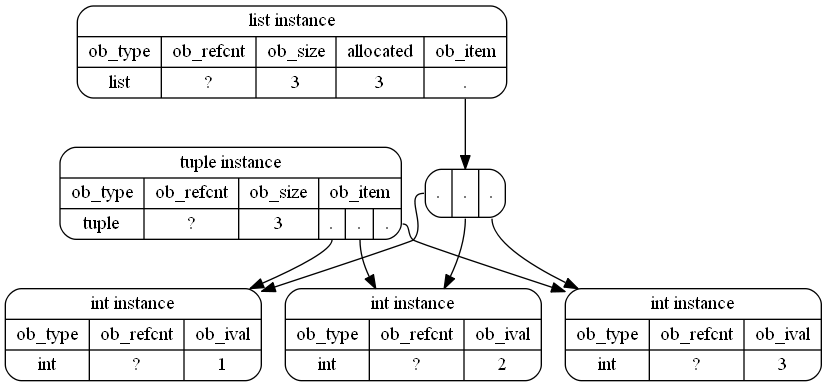
\includegraphics[width=300pt,height=160pt]{slike/img-list-tuple.png}
	\caption{Pojednostavljen prikaz memorijske organizacije liste i torke.}
	\label{fig:mem_list_org}
\end{figure}

U situacijama kada je unaprijed poznat maksimalan broj elemenata koji će se koristiti, često se kreira lista željene veličine:

\begin{minted}{python}
	lista = [None] * max_broj_elemenata
\end{minted}

Na ovaj način izbjegava se veliki broj naknadnih proširenja liste, što može pozitivno uticati na performanse programa.

\subsubsection*{Dodatne napomene}

Za razliku od klasičnih nizova u programskom jeziku \texttt{C}, liste u Pajtonu mogu sadržavati elemente različitih tipova:

\begin{minted}{python}
	lista = [1, "tekst", 3.14, True]
\end{minted}

Ova osobina čini liste veoma fleksibilnim i jednostavnim za upotrebu. Međutim, takva fleksibilnost ima svoju cijenu. Svaki element liste predstavlja zaseban Pajtonov objekat, koji pored stvarne vrijednosti sadrži i dodatne informacije, kao što su tip objekta i broj referenci na njega.

Interno posmatrano, lista ne sadrži same objekte već niz pokazivača na odgovarajuće objekte u memoriji. Zbog toga liste zauzimaju više memorijskog prostora nego homogeni nizovi implementirani u jezicima nižeg nivoa.

U većini praktičnih primjena liste predstavljaju osnovnu i najčešće korištenu strukturu podataka u Pajtonu. Zahvaljujući jednostavnoj sintaksi, podršci za dinamičko proširivanje i velikom broju ugrađenih metoda, one su često prvi izbor za organizaciju i obradu kolekcija podataka.

\subsection{Nizovi: modul \texttt{array}}

Pored lista, Pajton nudi i modul \texttt{array}, koji omogućava rad sa homogenim nizovima podataka. Po svojoj organizaciji i načinu korištenja, objekti tipa \texttt{array} slični su nizovima u programskim jezicima \textit{C} i \textit{C++}.

Za razliku od lista, koje mogu sadržavati elemente različitih tipova, svi elementi objekta \texttt{array} moraju biti istog tipa. Zbog toga se podaci mogu skladištiti efikasnije i zauzimati manje memorijskog prostora.

Elementi niza smješteni su u neprekidnom bloku memorije, što omogućava brz pristup proizvoljnom elementu korištenjem njegovog indeksa. Indeksiranje elemenata počinje od nule, kao i kod lista.

Prilikom kreiranja objekta tipa \texttt{array} potrebno je navesti oznaku tipa podataka (\textit{typecode}) koji će se skladištiti. Najčešće korištene oznake prikazane su u Tabeli~\ref{tab:TipPodatakaArray}.

\begin{table}[H]
	\caption{Najčešće korišteni tipovi podataka u modulu \texttt{array}.}
	\label{tab:TipPodatakaArray}
	\centering
	\begin{tabular}{llll}
		\hline
		\textbf{Typecode} & \textbf{Tip podatka} & \textbf{Pajtonov tip} & \textbf{Veličina (B)} \\
		\hline
		\texttt{'b'} / \texttt{'B'} & signed / unsigned char & int & 1 \\
		\texttt{'h'} / \texttt{'H'} & signed / unsigned short & int & 2 \\
		\texttt{'i'} / \texttt{'I'} & signed / unsigned int & int & 4 \\
		\texttt{'l'} / \texttt{'L'} & signed / unsigned long & int & 4 \\
		\texttt{'q'} / \texttt{'Q'} & signed / unsigned long long & int & 8 \\
		\texttt{'f'} & float & float & 4 \\
		\texttt{'d'} & double & float & 8 \\
		\hline
	\end{tabular}
\end{table}

Da bismo koristili modul \texttt{array}, potrebno ga je prethodno uključiti:

\begin{minted}{python}
	import array
\end{minted}

\subsubsection*{Inicijalizacija}

Objekat tipa \texttt{array} kreira se navođenjem oznake tipa i početnih vrijednosti:

\begin{minted}{python}
	from array import array
	
	my_array = array('i', [1, 2, 3, 4, 5])
\end{minted}

U ovom primjeru oznaka \texttt{'i'} označava cjelobrojne vrijednosti tipa \texttt{int}.

\subsubsection*{Osnovne operacije}

\begin{itemize}
	
	\item \textbf{Pristup elementima}
	
	\begin{minted}{python}
		print(my_array[0])   # 1
		print(my_array[2])   # 3
	\end{minted}
	
	\item \textbf{Izmjena elemenata}
	
	\begin{minted}{python}
		my_array[0] = 7
		print(my_array)
		# array('i', [7, 2, 3, 4, 5])
		
	\end{minted}
	
	\item \textbf{Dodavanje elementa na kraj niza}
	
	\begin{minted}{python}
		my_array.append(10)
	\end{minted}
	
	\item \textbf{Dodavanje više elemenata}
	
	\begin{minted}{python}
		from array import array
		
		floats = array('f', [2.0, 3.2, 1.4])
		floats.extend([1.1, 4.1, 5.2, 9.0])
	\end{minted}
	
	\item \textbf{Umetanje elementa}
	
	\begin{minted}{python}
		my_array.insert(2, 100)
	\end{minted}
	
	\item \textbf{Brisanje elementa}
	
	\begin{minted}{python}
		my_array.remove(100)
	\end{minted}
	
	\item \textbf{Uklanjanje posljednjeg elementa}
	
	\begin{minted}{python}
		my_array.pop()
	\end{minted}
	
\end{itemize}

\subsubsection*{Kada koristiti \texttt{array}?}

Modul \texttt{array} je posebno koristan kada radimo sa velikim kolekcijama numeričkih podataka istog tipa. U poređenju sa listama, objekti tipa \texttt{array} zauzimaju manje memorije i omogućavaju efikasnije skladištenje homogenih podataka.

Ipak, u naučnom računarstvu i analizi podataka danas se mnogo češće koriste strukture iz biblioteke \texttt{NumPy}, koje predstavljaju proširenje ideje homogenih nizova i nude znatno veće performanse i bogatiji skup funkcionalnosti.




\subsection{Rječnici}

Rječnik (\texttt{dict}) predstavlja jednu od najvažnijih ugrađenih struktura podataka u Pajtonu. Riječ je o promjenljivoj kolekciji elemenata organizovanih u obliku parova \emph{ključ--vrijednost}.

Za razliku od lista, gdje se elementima pristupa pomoću numeričkih indeksa, u rječnicima se pristup vrši preko ključeva. Svakom ključu pridružena je tačno jedna vrijednost, pri čemu ključevi moraju biti jedinstveni unutar rječnika.

Rječnici se često nazivaju i \textit{heš mapama} (eng. \textit{hash maps}), jer su interno implementirani korištenjem heš tabela.

\subsubsection*{Inicijalizacija}

Rječnik se može kreirati na više načina.

\begin{minted}{python}
	
	# Kreiranje pomoću vitičastih zagrada
	
	dct = {
		"ime": "Mirko",
		"godine": 30,
		"grad": "Banja Luka"
	}
	
	# Kreiranje pomoću konstruktora dict()
	
	dct1 = dict(
	ime="Mirko",
	godine=30,
	grad="Banja Luka"
	)
\end{minted}

\subsubsection*{Osnovne operacije}

\begin{itemize}
	
	\item \textbf{Pristup vrijednosti}
	
	Vrijednost pridružena određenom ključu dobija se korištenjem operatora \texttt{[]}.
	
	\begin{minted}{python}
		dct = {
			"ime": "Mirko",
			"godine": 30,
			"grad": "Banja Luka"
		}
		
		print(dct["ime"])      # Mirko
	\end{minted}
	
	\item \textbf{Dodavanje i izmjena elemenata}
	
	\begin{minted}{python}
		dct["godine"] = 31
	\end{minted}
	
	Ako ključ već postoji, njegova vrijednost se ažurira. U suprotnom se dodaje novi par ključ--vrijednost.
	
	\item \textbf{Brisanje elementa}
	
	Element se može ukloniti korištenjem ključne riječi \texttt{del} ili metode \texttt{pop()}.
	
	\begin{minted}{python}
		del dct["grad"]
	\end{minted}
	
	ili
	
	\begin{minted}{python}
		dct.pop("grad")
	\end{minted}
	
	\item \textbf{Provjera postojanja ključa}
	
	Operator \texttt{in} provjerava da li se određeni ključ nalazi u rječniku.
	
	\begin{minted}{python}
		print("ime" in dct)      # True
		print("pol" in dct)      # False
	\end{minted}
	
	\item \textbf{Iteriranje kroz rječnik}
	
	\begin{minted}{python}
		for kljuc, vrijednost in dct.items():
		print(kljuc, vrijednost)
	\end{minted}
	
	\item \textbf{Korisne metode}
	
	\begin{itemize}
		\item \texttt{len(dct)} -- vraća broj elemenata rječnika;
		\item \texttt{keys()} -- vraća kolekciju svih ključeva;
		\item \texttt{values()} -- vraća kolekciju svih vrijednosti;
		\item \texttt{items()} -- vraća parove (ključ, vrijednost);
		\item \texttt{get(kljuc)} -- sigurno dohvaća vrijednost bez generisanja greške ukoliko ključ ne postoji.
	\end{itemize}
	
\end{itemize}

\subsubsection*{Memorijska organizacija}

Rječnici su u Pajtonu implementirani korištenjem heš tabela. Osnovna ideja sastoji se u tome da se svaki ključ transformiše u cijeli broj primjenom heš funkcije. Dobijena vrijednost koristi se za brzo pronalaženje mjesta na kojem se nalazi odgovarajuća vrijednost.

Zahvaljujući ovakvoj organizaciji, osnovne operacije nad rječnicima imaju očekivanu vremensku složenost:

\begin{itemize}
	\item pristup elementu: $O(1)$,
	\item dodavanje elementa: $O(1)$,
	\item brisanje elementa: $O(1)$.
\end{itemize}

U najgorem slučaju ove operacije mogu biti sporije zbog pojave kolizija, ali se u praksi takve situacije rijetko javljaju.

Prilikom kreiranja rječnika interpreter rezerviše određeni broj mjesta u heš tabeli. Kako broj elemenata raste, tabela se po potrebi automatski proširuje kako bi se očuvala efikasnost pristupa.

Pojednostavljen prikaz organizacije rječnika dat je na Slici~\ref{fig:dict_mem_organization}.

\begin{figure}[H]
	\centering
	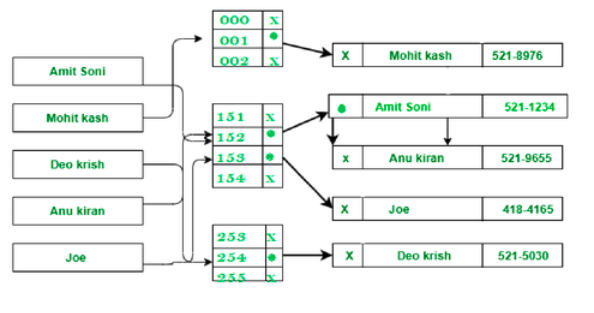
\includegraphics[width=300pt,height=160pt]{slike/dict_mem_organization.png}
	\caption{Pojednostavljen prikaz unutrašnje organizacije rječnika u Pajtonu.}
	\label{fig:dict_mem_organization}
\end{figure}

\subsubsection*{Dodatne napomene}

Ključevi u rječniku moraju biti nepromjenljivi objekti. Zbog toga se kao ključevi mogu koristiti objekti tipa \texttt{int}, \texttt{float}, \texttt{str} ili \texttt{tuple}, dok liste (\texttt{list}) ne mogu biti ključevi.

\begin{minted}{python}
	dct = {
		"ime": "Mirko",
		123: "identifikator",
		(1, 2): "par brojeva"
	}
\end{minted}

Zbog veoma brzog pristupa podacima, rječnici predstavljaju jednu od najčešće korištenih struktura podataka u modernom programiranju. Posebno su korisni kada je potrebno efikasno pretraživanje, grupisanje ili indeksiranje podataka.



\subsection{Skupovi}

Skup (\texttt{set}) predstavlja neuređenu kolekciju jedinstvenih elemenata. Po svojim osobinama odgovara matematičkom pojmu skupa: redoslijed elemenata nije važan, a duplikati nisu dozvoljeni.

Osnovna namjena skupova jeste efikasna provjera pripadnosti elementa kolekciji. Zbog toga se često koriste u algoritmima koji zahtijevaju brzo pretraživanje ili eliminisanje duplikata.

Elementi skupa mogu biti objekti nepromjenljivih tipova podataka, kao što su \texttt{int}, \texttt{float}, \texttt{str}, \texttt{tuple} ili \texttt{complex}. Sa druge strane, promjenljive kolekcije poput lista (\texttt{list}), rječnika (\texttt{dict}) i drugih skupova (\texttt{set}) ne mogu biti elementi skupa.

\subsubsection*{Inicijalizacija}

Skup se može kreirati na nekoliko načina:

\begin{minted}{python}
	skup = set()
	
	skup1 = {1, 2, 3, 4}
	
	skup2 = set((1, 2, "3"))
	
	skup3 = set([1, 2, 3])
\end{minted}

\textbf{Napomena.} Prazan skup se kreira pomoću funkcije \texttt{set()}. Izraz

\begin{minted}{python}
	skup = {}
\end{minted}

ne kreira prazan skup već prazan rječnik.

\subsubsection*{Osnovne metode}

\begin{itemize}
	
	\item \texttt{add(elem)} -- dodaje element u skup;
	
	\begin{minted}{python}
		skup.add(5)
	\end{minted}
	
	\item \texttt{remove(elem)} -- uklanja element iz skupa; generiše grešku ukoliko element ne postoji;
	
	\begin{minted}{python}
		skup.remove(5)
	\end{minted}
	
	\item \texttt{discard(elem)} -- uklanja element ako postoji, bez generisanja greške;
	
	\begin{minted}{python}
		skup.discard(5)
	\end{minted}
	
	\item \texttt{pop()} -- uklanja i vraća proizvoljan element skupa;
	
	\item \texttt{clear()} -- uklanja sve elemente iz skupa;
	
	\item \texttt{union()} ili operator \texttt{|} -- vraća uniju dva skupa;
	
	\begin{minted}{python}
		A = {1, 2, 3}
		B = {3, 4, 5}
		
		print(A | B)
		
		# {1, 2, 3, 4, 5}
		
	\end{minted}
	
	\item \texttt{intersection()} ili operator \texttt{\&} -- vraća presjek dva skupa;
	
	\begin{minted}{python}
		print(A & B)
		
		# {3}
		
	\end{minted}
	
	\item \texttt{difference()} ili operator \texttt{-} -- vraća razliku skupova;
	
	\begin{minted}{python}
		print(A - B)
		
		# {1, 2}
		
	\end{minted}
	
	\item Operator \texttt{in} koristi se za provjeru pripadnosti elementa skupu;
	
	\begin{minted}{python}
		print(3 in A)   # True
		print(7 in A)   # False
	\end{minted}
	
\end{itemize}

\subsubsection*{Memorijska organizacija}

Skupovi su u Pajtonu implementirani korištenjem heš tabela. Svakom elementu pridružuje se heš vrijednost koja omogućava veoma brzo pronalaženje njegove pozicije u memoriji.

Zahvaljujući takvoj organizaciji, osnovne operacije nad skupovima imaju očekivanu vremensku složenost:

\begin{itemize}
	\item dodavanje elementa: $O(1)$;
	\item uklanjanje elementa: $O(1)$;
	\item provjera pripadnosti: $O(1)$.
\end{itemize}

U najgorem slučaju, zbog pojave većeg broja kolizija, složenost može porasti na $O(n)$, ali se takve situacije u praksi rijetko javljaju.

Sljedeći primjer pokazuje da je skup predstavljen ugrađenim tipom podataka \texttt{set}:

\begin{minted}{python}
	s = {1, 2, 3}
	
	print(type(s))
	
	# <class 'set'>
	
\end{minted}

Pojednostavljen prikaz organizacije skupa dat je na Slici~\ref{fig:set_mem_organization}.

\begin{figure}[H]
	\centering
	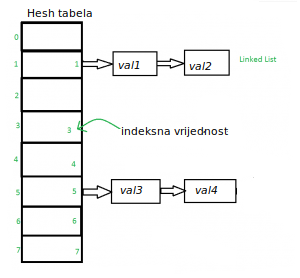
\includegraphics[width=220pt,height=150pt]{slike/set_mem_organization.png}
	\caption{Pojednostavljen prikaz unutrašnje organizacije skupa u Pajtonu.}
	\label{fig:set_mem_organization}
\end{figure}

\subsubsection*{Dodatne napomene}

Skupovi su naročito korisni kada je potrebno:

\begin{itemize}
	\item ukloniti duplikate iz kolekcije podataka;
	\item efikasno provjeriti da li se element nalazi u kolekciji;
	\item izvršavati skupovne operacije poput unije, presjeka i razlike.
\end{itemize}

Zbog veoma brzih operacija pretraživanja, skupovi predstavljaju jednu od najvažnijih struktura podataka u algoritmici i često se koriste za optimizaciju vremena izvršavanja programa.

\subsection{Torke}

Torka (\texttt{tuple}) predstavlja uređenu, indeksiranu i nepromjenljivu (\textit{immutable}) kolekciju elemenata. U Pajtonu se implementira pomoću ugrađenog tipa podataka \texttt{tuple}.

Za razliku od lista, elementi torke se ne mogu mijenjati nakon kreiranja objekta. Torke mogu sadržavati elemente različitih tipova podataka i dopuštaju pojavljivanje duplikata.

\subsubsection*{Inicijalizacija}

Torka se može kreirati na nekoliko načina:

\begin{minted}{python}
	my_tuple = ("aa", "bb", 2.0, 3)
	
	my_tuple1 = tuple(["abc", 3.2, "a"])
\end{minted}

Torka sa jednim elementom zahtijeva završni zarez:

\begin{minted}{python}
	t = (5,)
\end{minted}

Bez zareza izraz \texttt{(5)} predstavlja običan cjelobrojni objekat.

\subsubsection*{Osnovne operacije}

\begin{itemize}
	
	\item \textbf{Pristup elementima}
	
	Elementima torke pristupa se pomoću operatora \texttt{[]}:
	
	\begin{minted}{python}
		my_tuple = (1, 2, 3, 2, 4, 2, 5)
		
		print(my_tuple[2])   # 3
		print(my_tuple[-1])  # 5
	\end{minted}
	
	\item \textbf{Brojanje pojavljivanja elementa}
	
	Metoda \texttt{count()} vraća broj pojavljivanja elementa:
	
	\begin{minted}{python}
		my_tuple = (1, 2, 3, 2, 3, 5)
		
		print(my_tuple.count(2))  # 2
	\end{minted}
	
	\item \textbf{Pronalaženje indeksa elementa}
	
	Metoda \texttt{index()} vraća indeks prvog pojavljivanja elementa:
	
	\begin{minted}{python}
		print(my_tuple.index(2))  # 1
	\end{minted}
	
	\item \textbf{Dužina torke}
	
	Broj elemenata određuje se funkcijom \texttt{len()}:
	
	\begin{minted}{python}
		print(len(my_tuple))  # 6
	\end{minted}
	
	\item \textbf{Spajanje torki}
	
	Dvije torke mogu se spojiti operatorom \texttt{+}:
	
	\begin{minted}{python}
		t1 = ("a", "bb", 2)
		t2 = ("ee", 2, 3.4)
		t3 = t1 + t2
		print(t3)
		# ("a", "bb", 2, "ee", 2, 3.4)
		
	\end{minted}
	
	\item \textbf{Rezanje torke (slicing)}
	
	Kao i kod lista, moguće je izdvojiti dio torke:
	
	\begin{minted}{python}
		t = (0, 1, 2, 3, 4, 5)
		
		print(t[1:4])  # (1, 2, 3)
	\end{minted}
	
\end{itemize}

\subsubsection*{Memorijska organizacija}

Torke su nepromjenljive strukture podataka. Nakon kreiranja nije moguće dodavati, uklanjati niti mijenjati njihove elemente. Zbog toga Pajton može efikasnije upravljati memorijom nego kod promjenljivih struktura kao što su liste.

Objekat tipa \texttt{tuple} sadrži reference na svoje elemente. Pošto se broj elemenata ne može mijenjati nakon kreiranja torke, nije potrebno vršiti realokaciju memorije tokom izvršavanja programa.

Pristup elementima torke ostvaruje se direktnim indeksiranjem, pa je vremenska složenost operacije pristupa elementu jednaka $O(1)$.

Zbog svoje nepromjenljivosti, torke često zauzimaju manje memorije od lista sa istim brojem elemenata i mogu se koristiti kao ključevi u rječnicima ili kao elementi skupova, pod uslovom da svi njihovi elementi takođe budu nepromjenljivi.

Poređenje memorijske organizacije lista i torki prikazano je na Slici~\ref{fig:mem_list_org}.

\subsubsection*{Kada koristiti torke?}

Torke su pogodan izbor kada:

\begin{itemize}
	\item podaci ne treba da se mijenjaju nakon kreiranja;
	\item želimo smanjiti potrošnju memorije;
	\item želimo koristiti kolekciju kao ključ u rječniku ili element skupa;
	\item želimo jasno naglasiti da određeni skup podataka predstavlja jednu logičku cjelinu.
\end{itemize}

Tipični primjeri upotrebe su predstavljanje koordinata tačke, datuma, RGB boja i drugih nepromjenljivih zapisa podataka.

\section{Funkcije}

Funkcije predstavljaju jedan od osnovnih mehanizama za organizaciju programa. Njihova uloga je da složen problem podijele na manje, logički zaokružene cjeline koje se mogu višestruko koristiti.

U Pajtonu je svaka funkcija objekat. To znači da se funkcija može dodijeliti varijabli, proslijediti kao argument drugoj funkciji ili vratiti kao rezultat izvršavanja funkcije. Kada interpreter obradi definiciju funkcije, kreira se objekat tipa \texttt{function} koji sadrži informacije o nazivu funkcije, parametrima, tijelu funkcije i drugim metapodacima.

Funkcija se definiše pomoću ključne riječi \texttt{def}. Nakon naziva funkcije navode se parametri u zagradama, a tijelo funkcije se piše u uvučenom bloku koda. Naredba \texttt{return} služi za vraćanje rezultata i završetak izvršavanja funkcije.

\begin{minted}{python}
	def proizvod_brojeva(x, y):
	proizvod = x * y
	return proizvod
\end{minted}

Funkcija se poziva navođenjem njenog naziva i odgovarajućih argumenata:

\begin{minted}{python}
	rezultat = proizvod_brojeva(4, 3)
	
	print(rezultat)  # 12
\end{minted}

\subsection*{Podrazumijevane vrijednosti parametara}

Parametrima funkcije mogu se dodijeliti podrazumijevane vrijednosti koje će biti korištene ukoliko korisnik ne navede odgovarajući argument.

\begin{minted}{python}
	def umnozi(tekst="Mirko", broj_ponavljanja=1):
	print(tekst * broj_ponavljanja)
	
	umnozi()
\end{minted}

U ovom slučaju ispisuje se:

\begin{minted}{text}
	Mirko
\end{minted}

jer se koriste podrazumijevane vrijednosti parametara.

\subsection*{Promjenljiv broj argumenata}

Pajton omogućava definisanje funkcija koje prihvataju proizvoljan broj pozicionih ili imenovanih argumenata.

Operator \texttt{*} sakuplja dodatne pozicione argumente u torku:

\begin{minted}{python}
	def ispisi_brojeve(*brojevi):
	    for broj in brojevi:
	        print(broj)
\end{minted}

Operator \texttt{**} sakuplja imenovane argumente u rječnik:

\begin{minted}{python}
	def ispisi_podatke(**podaci):
	    for kljuc, vrijednost in podaci.items():
	        print(kljuc, ":", vrijednost)
	#main
	ispisi_podatke(
	    ime="Mirko",
	    prezime="Marković"
	)
\end{minted}

\subsection*{Vraćanje više vrijednosti}

Funkcija može vratiti više vrijednosti odjednom. U pozadini se takve vrijednosti pakuju u torku.

\begin{minted}{python}
	def podjela(x, y):
	    kolicnik = x // y
	    ostatak = x % y
	
	    return kolicnik, ostatak
	#main
	k, o = podjela(10, 3)
	print(k, o)  # 3 1
\end{minted}

\subsection*{Prosljeđivanje argumenata}

U Pajtonu se funkcijama prosljeđuje referenca na objekat. Zbog toga ponašanje zavisi od toga da li je objekat promjenljiv ili nepromjenljiv.

Promjenljivi objekti (liste, rječnici i skupovi) mogu biti izmijenjeni unutar funkcije:

\begin{minted}{python}
	def dodaj_element(lista, element):
	
	    lista.append(element)
	
	#main
	brojevi = [1, 2, 3]
	dodaj_element(brojevi, 5)
	print(brojevi)  # [1, 2, 3, 5]
	
\end{minted}

Pošto funkcija i pozivalac referenciraju isti objekat liste, promjena je vidljiva i nakon povratka iz funkcije.

Ako želimo izbjeći izmjenu originalne liste, potrebno je funkciji proslijediti kopiju:

\begin{minted}{python}
	dodaj_element(brojevi.copy(), 5)
\end{minted}

\subsection*{Nepromjenljivi objekti}

Cijeli brojevi, decimalni brojevi, stringovi i torke predstavljaju nepromjenljive objekte. Njihova izmjena zapravo podrazumijeva kreiranje novog objekta.

\begin{minted}{python}
	def inkrementiraj(x):
	    x += 1
	    print("Unutar funkcije:", x)
	
	#main
	y = 5	
	inkrementiraj(y)
	print(y)
\end{minted}

Rezultat izvršavanja je:
\begin{minted}{text}
	Unutar funkcije: 6
	5
\end{minted}

Vrijednost varijable \texttt{y} ostaje nepromijenjena jer izraz \texttt{x += 1} kreira novi objekat i lokalna varijabla \texttt{x} počinje da referencira taj novi objekat.

\subsection*{Globalne varijable}

Ključna riječ \texttt{global} omogućava izmjenu globalne varijable unutar funkcije.

\begin{minted}{python}
	def my_func():
	    global x
	    x = 10
	#main
	x = 20
	my_func()
	print(x)  # 10
\end{minted}
Ipak, prekomjerna upotreba globalnih varijabli se ne preporučuje jer otežava razumijevanje i održavanje programa.

\subsection*{Funkcije kao argumenti}

Pošto su funkcije objekti, mogu se prosljeđivati drugim funkcijama kao argumenti.

\begin{minted}{python}
	def saberi(a, b):
	    return a + b
	
	def primijeni(funkcija, x, y):
	    return funkcija(x, y)
	
	#main
	rezultat = primijeni(saberi, 2, 3)
	print(rezultat)  # 5
\end{minted}

Ovakav pristup predstavlja osnovu mnogih naprednih tehnika programiranja, uključujući funkcionalno programiranje i rad sa bibliotekama za obradu podataka.


\textit{Anonimne funkcije.} Anonimne funkcije definišu se pomoću ključne riječi \texttt{lambda}, zbog čega se često nazivaju i \textit{lambda funkcije}. Naziv „anonimne“ potiče od činjenice da se funkcija može definisati bez eksplicitnog navođenja njenog imena, za razliku od standardnih funkcija koje se definišu pomoću ključne riječi \texttt{def}.

Opšta sintaksa lambda funkcije je:

\begin{minted}{python}
	lambda argumenti: izraz
\end{minted}

Pri tome, \textit{argumenti} predstavljaju ulazne parametre funkcije, dok \textit{izraz} definiše operaciju koja se izvršava nad tim parametrima. Vrijednost izraza automatski predstavlja rezultat funkcije.

Sljedeći primjer definiše lambda funkciju za sabiranje dva broja:

\begin{minted}{python}
	suma = lambda x, y: x + y
	print(suma(4, 3))  # Output: 7
\end{minted}

U ovom primjeru lambda funkcija je dodijeljena varijabli \texttt{suma}. To je moguće zato što su funkcije u Pajtonu objekti, pa se mogu čuvati u varijablama, prosljeđivati drugim funkcijama ili vraćati kao rezultat izvršavanja funkcije.

Lambda funkcije su naročito korisne kada je potrebno definisati kratku funkciju koja se koristi samo na jednom mjestu u programu. U takvim situacijama često nije potrebno uvoditi funkciju sa punim imenom.

Na primjer, prethodna funkcija može se pozvati direktno:

\begin{minted}{python}
	print((lambda x, y: x + y)(4, 3))
\end{minted}

Iako lambda funkcije mogu imati proizvoljan broj parametara, njihovo tijelo mora sadržavati samo jedan izraz. Zbog toga se uglavnom koriste za jednostavne operacije.

Lambda funkcije se često kombinuju sa ugrađenim funkcijama za obradu kolekcija, kao što su \texttt{map()}, \texttt{filter()} i \texttt{reduce()}. O ovim funkcijama biće više riječi u nastavku knjige, u Sekciji~\ref{sec:concepts-pyhton}.


\section{Neki programski koncepti i ugrađene funkcije}
\label{sec:concepts-pyhton}

U ovoj sekciji predstavljamo nekoliko važnih koncepata i ugrađenih funkcija koje se često koriste u programskom jeziku Pajton. Posebna pažnja posvećena je komprehenziji liste (\textit{list comprehension}) i funkcijama \texttt{map()}, \texttt{filter()} i \texttt{reduce()}, koje omogućavaju sažetije i preglednije pisanje programa te uvode određene elemente funkcionalnog programiranja.

\subsection{Komprehenzija liste}

Komprehenzija liste (\textit{list comprehension}) predstavlja koncizan način kreiranja i popunjavanja lista. Omogućava formiranje nove liste u jednoj naredbi, bez potrebe za eksplicitnim korištenjem petlji i metoda za dodavanje elemenata.

Osnovna sintaksa je:

\begin{minted}{python}
	lista = [izraz for element in iterabilni_objekat]
\end{minted}

Pri tome:

\begin{itemize}
	\item \textit{izraz} definiše vrijednost koja se upisuje u novu listu;
	\item \textit{element} predstavlja trenutni element iterabilnog objekta;
	\item \textit{iterabilni\_objekat} može biti lista, torka, skup, string, generator ili drugi iterabilni objekat.
\end{itemize}

Na primjer, listu prvih deset parnih brojeva možemo kreirati na sljedeći način:

\begin{minted}{python}
	parni = [2 * i for i in range(1, 11)]
\end{minted}

Isti rezultat mogao bi se dobiti i pomoću klasične petlje:

\begin{minted}{python}
	parni = []
	for i in range(1, 11):
	    parni.append(2 * i)
\end{minted}

Komprehenzija liste može sadržavati i uslov:

\begin{minted}{python}
	lista = [izraz for element in iterabilni_objekat if uslov]
\end{minted}

Na primjer, izdvajanje parnih brojeva iz liste:

\begin{minted}{python}
	brojevi = [1, 2, 3, 4, 5, 6]
	parni = [x for x in brojevi if x % 2 == 0]
	print(parni)  # [2, 4, 6]
\end{minted}

Komprehenzija liste često rezultira kraćim i preglednijim kodom, posebno kod jednostavnih transformacija i filtriranja podataka.

\subsection{Funkcije \texttt{map()}, \texttt{filter()} i \texttt{reduce()}}

Funkcije \texttt{map()}, \texttt{filter()} i \texttt{reduce()} predstavljaju osnovne alate funkcionalnog programiranja. Njihova primjena omogućava obradu kolekcija podataka bez eksplicitnog pisanja petlji.

\subsubsection*{Funkcija \texttt{map()}}

Funkcija \texttt{map()} prima funkciju i iterabilni objekat te primjenjuje zadatu funkciju na svaki element kolekcije.

\begin{minted}{python}
	brojevi = [1, 2, 3, 4, 5]
	dupli = map(lambda x: 2 * x, brojevi)
	print(list(dupli)) 	# [2, 4, 6, 8, 10]
	
\end{minted}

U Pythonu 3 funkcija \texttt{map()} vraća iterator, pa je često potrebno rezultat pretvoriti u listu pozivom funkcije \texttt{list()}.

\subsubsection*{Funkcija \texttt{filter()}}

Funkcija \texttt{filter()} služi za izdvajanje elemenata koji zadovoljavaju određeni uslov.

\begin{minted}{python}
	brojevi = [1, 2, 3, 4, 5, 6]
	
	parni = filter(lambda x: x % 2 == 0, brojevi)
	print(list(parni))  # [2, 4, 6]
	
\end{minted}

Funkcija koja se prosljeđuje kao prvi argument mora vraćati logičku vrijednost (\texttt{True} ili \texttt{False}).

\subsubsection*{Funkcija \texttt{reduce()}}

Funkcija \texttt{reduce()} sukcesivno kombinuje elemente kolekcije primjenom zadate funkcije.

Njena opšta sintaksa je:
\begin{minted}{python}
	reduce(funkcija, iterable[, pocetna_vrijednost])
\end{minted}

Funkcija \texttt{reduce()} nije ugrađena u osnovni skup funkcija jezika Pajton, već se nalazi u modulu \texttt{functools}.

\begin{minted}{python}
	from functools import reduce
	
	brojevi = [1, 2, 3, 4, 5]
	
	proizvod = reduce(
	    lambda x, y: x * y,
	    brojevi,
	    1)
	
	print(proizvod) # 120
\end{minted}

U ovom primjeru izvršavaju se sljedeće operacije:

\begin{align*}
	1 \cdot 1 &= 1,\\
	1 \cdot 2 &= 2,\\
	2 \cdot 3 &= 6,\\
	6 \cdot 4 &= 24,\\
	24 \cdot 5 &= 120.
\end{align*}

Dakle, funkcija \texttt{reduce()} „redukuje“ čitavu kolekciju na jednu konačnu vrijednost.

\subsection*{Poređenje sa komprehenzijom liste}

U savremenom Pajtonu mnoge operacije realizovane funkcijama \texttt{map()} i \texttt{filter()} često se zapisuju pomoću komprehenzije liste, jer je takav kod pregledniji. Na primjer:

\begin{minted}{python}
	parni = [x for x in brojevi if x % 2 == 0]
\end{minted}

predstavlja alternativu izrazu

\begin{minted}{python}
	parni = filter(lambda x: x % 2 == 0, brojevi)
\end{minted}

Izbor između ova dva pristupa najčešće zavisi od stila programiranja i složenosti konkretnog problema.


\subsection{Funkcije \texttt{zip()}, \texttt{enumerate()} i \texttt{sort()}}

Funkcije \texttt{zip()} i \texttt{enumerate()} spadaju među najčešće korištene ugrađene funkcije za obradu i iteriranje kroz kolekcije podataka.

\subsubsection*{Funkcija \texttt{zip()}}

Funkcija \texttt{zip()} prima dva ili više iterabilnih objekata i vraća iterator koji generiše torke sastavljene od odgovarajućih elemenata tih objekata.

Njena opšta sintaksa je:

\begin{minted}{python}
	zip(iterable1, iterable2, ...)
\end{minted}

gdje su \textit{iterable1}, \textit{iterable2}, \ldots proizvoljni iterabilni objekti. Na primjer:

\begin{minted}{python}
	lista1 = [1, 2, 3, 4]
	lista2 = [5, 6, 7, 8]
	parovi = zip(lista1, lista2)
	
	print(list(parovi))
	# [(1, 5), (2, 6), (3, 7), (4, 8)]
	
\end{minted}

Funkcija \texttt{zip()} zaustavlja generisanje parova čim se iscrpi najkraći od proslijeđenih iterabilnih objekata.

\subsubsection*{Funkcija \texttt{enumerate()}}

Funkcija \texttt{enumerate()} omogućava istovremeno pristupanje elementima kolekcije i njihovim indeksima.

Sintaksa funkcije je:

\begin{minted}{python}
	enumerate(iterable, start=0)
\end{minted}

gdje je:

\begin{itemize}
	\item \textit{iterable} iterabilni objekat;
	\item \textit{start} početna vrijednost indeksa (podrazumijevano je 0).
\end{itemize}

Primjer:

\begin{minted}{python}
	voce = ["jabuka", "banana", "kruška", "breskva"]
	
	for i, vocka in enumerate(voce):
	    print(i, vocka)
\end{minted}

Rezultat izvršavanja je:

\begin{minted}{text}
	0 jabuka
	1 banana
	2 kruška
	3 breskva
\end{minted}

Funkcija \texttt{enumerate()} često predstavlja pregledniju alternativu ručnom vođenju brojača unutar petlje.

\subsubsection*{Sortiranje lista}

Pajton omogućava sortiranje elemenata pomoću metode \texttt{sort()} i ugrađene funkcije \texttt{sorted()}.

Metoda \texttt{sort()} sortira postojeću listu direktno u memoriji.

Njena sintaksa je:

\begin{minted}{python}
	lista.sort(reverse=False, key=None)
\end{minted}

Parametar \texttt{reverse} određuje redoslijed sortiranja:

\begin{itemize}
	\item \texttt{False} -- rastući poredak (podrazumijevano);
	\item \texttt{True} -- opadajući poredak.
\end{itemize}

Parametar \texttt{key} omogućava zadavanje funkcije koja određuje kriterijum sortiranja. U nastavku slijedi jedan primjer. 

\begin{minted}{python}
	brojevi = [6, 3, 8, 3, 1, 7]
	brojevi.sort(reverse=True)
	print(brojevi) # [8, 7, 6, 3, 3, 1]
	
\end{minted}

Ako elementi liste nisu međusobno uporedivi, javlja se greška:

\begin{minted}{python}
	TypeError: '<' not supported between
	instances of 'str' and 'int'
\end{minted}

\subsubsection*{Funkcija \texttt{sorted()}}

Za razliku od metode \texttt{sort()}, funkcija \texttt{sorted()} ne mijenja originalnu kolekciju, već vraća novu sortiranu kolekciju.

\begin{minted}{python}
	brojevi = [5, 2, 8, 3, 1, 7]
	sortirani = sorted(brojevi)
	print(sortirani)
	# [1, 2, 3, 5, 7, 8]
	print(brojevi)
	# [5, 2, 8, 3, 1, 7]
	
\end{minted}

U praksi se \texttt{sort()} koristi kada želimo izmijeniti postojeću listu, dok se \texttt{sorted()} koristi kada je potrebno sačuvati originalni redoslijed elemenata.

\subsubsection*{Neke često korištene ugrađene funkcije}

Pored navedenih funkcija, Pajton sadrži veliki broj korisnih ugrađenih funkcija. Neke od najčešće korištenih su:

\begin{itemize}
	\item \texttt{sum(iterable)} -- vraća sumu elemenata iterabilnog objekta;
	\item \texttt{max(iterable)} -- vraća najveći element;
	\item \texttt{min(iterable)} -- vraća najmanji element;
	\item \texttt{abs(x)} -- vraća apsolutnu vrijednost broja;
	\item \texttt{round(x, n)} -- zaokružuje broj na \texttt{n} decimalnih mjesta;
	\item \texttt{len(obj)} -- vraća broj elemenata kolekcije;
	\item \texttt{eval(expr)} -- izračunava izraz zapisan u obliku stringa.
\end{itemize}

\section{Moduli}

\textit{Modul} predstavlja datoteku koja sadrži definicije funkcija, klasa, promjenljivih i drugih programskih elemenata. Naziv modula odgovara nazivu datoteke sa ekstenzijom \texttt{.py}.

Moduli omogućavaju organizovanje programa u manje cjeline i ponovnu upotrebu koda u različitim projektima.

Da bismo koristili modul, potrebno ga je prvo uključiti pomoću naredbe \texttt{import}.

Na primjer, ako postoji datoteka \texttt{mojmodul.py}, modul se uključuje na sljedeći način:

\begin{minted}{python}
	import mojmodul
\end{minted}

Nakon toga funkcijama, klasama i promjenljivama modula pristupamo pomoću tačkaste notacije:

\begin{minted}{python}
	mojmodul.moja_funkcija()
\end{minted}

Moguće je uvesti i samo određene elemente modula:

\begin{minted}{python}
	from mojmodul import moja_funkcija
\end{minted}

Tada se funkcija može pozivati direktno:

\begin{minted}{python}
	moja_funkcija()
\end{minted}

Moduli predstavljaju jedan od osnovnih mehanizama organizacije programa u Pajtonu i omogućavaju razvoj većih i preglednijih softverskih sistema.


Pajton dolazi sa velikim brojem ugrađenih modula, među kojima se posebno izdvajaju \texttt{math}, \texttt{random}, \texttt{datetime} i \texttt{os}. Pored njih, u praksi se često koriste i brojni eksterni moduli i biblioteke, kao što je \texttt{numpy}, o kojima će biti više riječi u nastavku ovog poglavlja.

Moduli koji su dio standardne biblioteke dostupni su odmah nakon instalacije Pajtona i nije ih potrebno dodatno instalirati. Sa druge strane, za korištenje eksternih modula potrebno ih je prethodno instalirati.

Instalacija eksternih modula najčešće se vrši pomoću menadžera paketa \texttt{pip}, koji se standardno isporučuje uz većinu Pajton instalacija. Da bismo instalirali određeni modul, na terminalu izvršimo naredbu:

\begin{minted}{bash}
	pip install naziv_modula
\end{minted}

gdje \texttt{naziv\_modula} predstavlja naziv modula koji želimo instalirati.

Na primjer, za instalaciju modula \texttt{requests} koristimo naredbu:

\begin{minted}{bash}
	pip install requests
\end{minted}

Nakon pokretanja naredbe, \texttt{pip} automatski preuzima traženi paket sa repozitorijuma PyPI (\emph{Python Package Index}) i instalira ga u trenutno Pajton okruženje.

PyPI predstavlja centralni repozitorijum Pajton paketa i sadrži stotine hiljada biblioteka koje su slobodno dostupne za korištenje. Zahvaljujući njemu, funkcionalnost jezika može se značajno proširiti bez potrebe za implementacijom svega od početka.

Nakon uspješne instalacije, modul se može uključiti u program pomoću naredbe \texttt{import}:

\begin{minted}{python}
	import requests
\end{minted}

Ponekad je potrebno instalirati tačno određenu verziju modula. To se postiže navođenjem broja verzije iza operatora \texttt{==}. Na primjer, za instalaciju verzije 2.2.1 modula \texttt{requests} koristimo:

\begin{minted}{bash}
	pip install requests==2.2.1
\end{minted}

Informacije o instaliranim modulima mogu se prikazati naredbom:

\begin{minted}{bash}
	pip list
\end{minted}

dok se detaljne informacije o konkretnom modulu dobijaju naredbom:

\begin{minted}{bash}
	pip show requests
\end{minted}

Savremeni Pajton projekti često koriste virtuelna okruženja (\emph{virtual environments}) kako bi se zavisnosti različitih projekata držale odvojeno. O ovom konceptu biće više riječi u kasnijim poglavljima.

\subsection{Modul \texttt{math}}

Modul \texttt{math} sadrži veliki broj matematičkih funkcija i konstanti koje se često koriste u naučnom računarstvu, obradi podataka i razvoju algoritama.

Prije korištenja potrebno ga je uključiti naredbom:

\begin{minted}{python}
	import math
\end{minted}

Nakon toga funkcijama i konstantama modula pristupa se preko prefiksa \texttt{math}.

\begin{minted}{python}
	import math
	
	# Kvadratni korijen
	
	x = math.sqrt(25)
	print(x)      # 5.0
	
	# Konstanta pi
	
	print(math.pi)
	
	# Sinus ugla od 45 stepeni
	
	print(math.sin(math.radians(45)))
\end{minted}

Napomenimo da trigonometrijske funkcije modula \texttt{math} očekuju argument izražen u radijanima. Zbog toga se za pretvaranje stepeni u radijane često koristi funkcija \texttt{math.radians()}.

Neke od najčešće korištenih funkcija modula \texttt{math} su:

\begin{itemize}
	\item \texttt{sqrt(x)} -- kvadratni korijen broja;
	\item \texttt{pow(x,y)} -- stepenovanje;
	\item \texttt{log(x)} -- prirodni logaritam;
	\item \texttt{log10(x)} -- dekadni logaritam;
	\item \texttt{exp(x)} -- vrijednost $e^x$;
	\item \texttt{floor(x)} -- zaokruživanje naniže;
	\item \texttt{ceil(x)} -- zaokruživanje naviše;
	\item \texttt{fabs(x)} -- apsolutna vrijednost;
	\item \texttt{gcd(a,b)} -- najveći zajednički djelilac;
	\item \texttt{dist(p,q)} -- Euklidovo rastojanje između dvije tačke;
	\item \texttt{sin(x)}, \texttt{cos(x)}, \texttt{tan(x)} -- trigonometrijske funkcije.
\end{itemize}

Pored funkcija, modul sadrži i korisne matematičke konstante kao što su \texttt{math.pi} i \texttt{math.e}.

\subsection{Modul \texttt{random}}

Modul \texttt{random} omogućava generisanje pseudo-slučajnih brojeva i slučajan izbor elemenata iz kolekcija podataka.

Uključuje se naredbom:

\begin{minted}{python}
	import random
\end{minted}

Neke od najčešće korištenih funkcija su:

\begin{itemize}
	\item \texttt{random()} -- generiše realan broj iz intervala $[0,1)$;
	\item \texttt{randint(a,b)} -- generiše slučajan cijeli broj između $a$ i $b$ (uključujući granice);
	\item \texttt{choice(seq)} -- vraća slučajno odabrani element kolekcije;
	\item \texttt{shuffle(seq)} -- nasumično permutuje elemente liste;
	\item \texttt{sample(population,k)} -- bira $k$ različitih elemenata bez ponavljanja;
	\item \texttt{seed(x)} -- postavlja početno stanje generatora slučajnih brojeva.
\end{itemize}

Primjer korištenja:

\begin{minted}{python}
	import random
	
	print(random.random())
	print(random.randint(1, 10))
	
	imena = ["Ana", "Marko", "Petar"]
	print(random.choice(imena))
\end{minted}

Generator slučajnih brojeva u modulu \texttt{random} zasniva se na determinističkom algoritmu. To znači da se za isto početno stanje, zadato funkcijom \texttt{seed()}, uvijek generiše isti niz vrijednosti. Ova osobina je posebno korisna pri testiranju programa i reprodukciji eksperimenata.

Iako se generisane vrijednosti ponašaju kao slučajne, one nisu pogodne za kriptografske primjene. Za potrebe kriptografije koristi se modul \texttt{secrets}, koji generiše kriptografski sigurne slučajne vrijednosti.


\subsection{Modul \texttt{time}}

Modul \texttt{time} predstavlja dio standardne Pajton biblioteke i omogućava rad sa vremenom. Njegove funkcije koriste se za mjerenje trajanja izvršavanja programa, dobijanje trenutnog vremena, privremeno zaustavljanje izvršavanja programa i konverziju između različitih vremenskih formata.

Modul se uključuje naredbom:

\begin{minted}{python}
	import time
\end{minted}

Neke od najčešće korištenih funkcija su:

\begin{itemize}
	\item \texttt{time()} -- vraća trenutno vrijeme izraženo kao broj sekundi proteklih od 1. januara 1970. godine (tzv. Unix epoha);
	
	\item \texttt{sleep(secs)} -- privremeno zaustavlja izvršavanje programa na zadati broj sekundi;
	
	\item \texttt{localtime([secs])} -- pretvara vrijeme izraženo u sekundama od epohe u lokalni datum i vrijeme;
	
	\item \texttt{ctime([secs])} -- vraća tekstualni prikaz datuma i vremena;
	
	\item \texttt{perf\_counter()} -- vraća precizan brojač vremena koji se često koristi za mjerenje vremena izvršavanja algoritama.
	
\end{itemize}

Primjer:

\begin{minted}{python}
	import time
	print(time.time())
	time.sleep(2)
	print("Program nastavljen.")
\end{minted}

\subsection{Modul \texttt{os}}

Modul \texttt{os} omogućava interakciju sa operativnim sistemom. Njegove funkcije koriste se za rad sa datotekama i direktorijumima, pristup varijablama okruženja i izvršavanje određenih sistemskih operacija.

Modul se uključuje naredbom:

\begin{minted}{python}
	import os
\end{minted}

Neke od najčešće korištenih funkcija i atributa su:

\begin{itemize}
	\item \texttt{os.name} -- vraća oznaku operativnog sistema;
	
	\item \texttt{os.getcwd()} -- vraća trenutni radni direktorijum;
	
	\item \texttt{os.chdir(path)} -- mijenja trenutni radni direktorijum;
	
	\item \texttt{os.listdir(path)} -- vraća listu datoteka i direktorijuma;
	
	\item \texttt{os.mkdir(path)} -- kreira novi direktorijum;
	
	\item \texttt{os.makedirs(path)} -- kreira direktorijum zajedno sa svim potrebnim poddirektorijumima;
	
	\item \texttt{os.remove(path)} -- briše datoteku;
	
	\item \texttt{os.rmdir(path)} -- briše prazan direktorijum;
	
	\item \texttt{os.rename(src, dest)} -- mijenja naziv datoteke ili direktorijuma;
	
	\item \texttt{os.path.exists(path)} -- provjerava da li putanja postoji;
	
	\item \texttt{os.path.isfile(path)} -- provjerava da li putanja predstavlja datoteku;
	
	\item \texttt{os.path.isdir(path)} -- provjerava da li putanja predstavlja direktorijum.
	
\end{itemize}

Primjer:

\begin{minted}{python}
	import os
	
	print(os.getcwd())
	if os.path.exists("podaci.txt"):
	    print("Datoteka postoji.")
\end{minted}

\subsection{Modul \texttt{copy}}

Modul \texttt{copy} omogućava pravljenje kopija objekata. Posebno je koristan pri radu sa složenim strukturama podataka, kao što su liste, rječnici i ugniježđene kolekcije.

Modul podržava dvije osnovne vrste kopiranja:

\begin{itemize}
	\item \textbf{površinsko kopiranje} (\emph{shallow copy});
	\item \textbf{dubinsko kopiranje} (\emph{deep copy}).
\end{itemize}

Modul se uključuje naredbom:

\begin{minted}{python}
	import copy
\end{minted}

\subsubsection*{Površinsko kopiranje}

Funkcija \texttt{copy()} kreira novi objekat, ali elementi koji se nalaze unutar njega ostaju zajednički sa originalnim objektom.

\begin{minted}{python}
	import copy
	
	originalna_lista = [1, [2, 3], 4]
	kopija = copy.copy(originalna_lista)
	kopija[1][0] = 99
	print(originalna_lista) # [1, [99, 3], 4]
\end{minted}

Vidimo da je izmjena u unutrašnjoj listi vidljiva i u originalnom objektu.

\subsubsection*{Dubinsko kopiranje}

Funkcija \texttt{deepcopy()} rekurzivno kopira sve objekte sadržane unutar originalnog objekta, čime nastaje potpuno nezavisna kopija.

\begin{minted}{python}
	import copy
	
	originalna_lista = [1, [2, 3], 4]
	kopija = copy.deepcopy(originalna_lista)
	kopija[1][0] = 99
	print(originalna_lista) # [1, [2, 3], 4]
\end{minted}

U ovom slučaju promjene napravljene nad kopijom ne utiču na originalni objekat.

\bigskip

Površinsko kopiranje je brže i troši manje memorije, dok dubinsko kopiranje zahtijeva više vremena i memorijskog prostora, ali garantuje potpunu nezavisnost kopije od originalnog objekta.
  

\section{Izuzeci}

Tokom izvršavanja programa mogu se pojaviti različite greške koje nije moguće otkriti u fazi prevođenja programa. Takve greške nazivaju se \textit{izuzeci} (engl. \textit{exceptions}).

Tipični primjeri izuzetaka su:

\begin{itemize}
	\item dijeljenje brojem nula;
	\item pristup nepostojećoj datoteci;
	\item pokušaj konverzije neispravnog podatka;
	\item pristup elementu izvan granica kolekcije;
	\item korištenje objekta neodgovarajućeg tipa.
\end{itemize}

Mehanizam izuzetaka omogućava programu da prepozna nastalu grešku i na nju reaguje na kontrolisan način, umjesto da se izvršavanje trenutno prekine.

\subsection{Blok \texttt{try-except}}

Osnovni mehanizam za obradu izuzetaka u Pajtonu zasniva se na konstrukciji \texttt{try-except}. K\^od koji potencijalno može izazvati izuzetak smješta se u blok \texttt{try}, dok se obrada greške definiše u odgovarajućem bloku \texttt{except}.

Opšti oblik ove konstrukcije je:

\begin{minted}{python}
	try:
	    # kod koji može izazvati izuzetak
	except ExceptionType:
	    # obrada izuzetka
\end{minted}

Na primjer:

\begin{minted}{python}
	try:
	    x = 10 / 0
	except ZeroDivisionError:
	    print("Dijeljenje nulom nije dozvoljeno.")
\end{minted}

U ovom slučaju program neće biti prekinut, već će se izvršiti odgovarajuća poruka o grešci.

\subsection{Hvatanje više vrsta izuzetaka}

Jedan blok \texttt{try} može imati više blokova \texttt{except}, pri čemu svaki obrađuje određenu vrstu greške.

\begin{minted}{python}
	try:
	    # kod koji može izazvati izuzetak
	except ValueError:
	    print("Greška u vrijednosti.")
	except TypeError:
	    print("Greška u tipu podatka.")
	except Exception:
	    print("Dogodio se neočekivani izuzetak.")
\end{minted}

Klasa \texttt{Exception} predstavlja baznu klasu većine izuzetaka i često se koristi za hvatanje svih neobrađenih grešaka.

\subsection{Generisanje izuzetaka}

Pored hvatanja postojećih izuzetaka, moguće je i eksplicitno generisati izuzetak pomoću naredbe \texttt{raise}.

\begin{minted}{python}
	raise ValueError("Neispravan ulazni podatak.")
\end{minted}

Ovakav pristup je koristan kada želimo da sami signaliziramo pojavu greške ili neispravnog stanja u programu.

\subsection{Blok \texttt{finally}}

Ponekad je potrebno izvršiti određeni kod bez obzira na to da li je došlo do izuzetka ili ne. Za tu svrhu koristi se blok \texttt{finally}.

\begin{minted}{python}
	try:
	    # kod koji može izazvati izuzetak
	finally:
	    # kod koji se uvijek izvršava
\end{minted}

Blok \texttt{finally} često se koristi za zatvaranje datoteka, oslobađanje resursa ili izvršavanje operacija čišćenja nakon završetka rada programa.

\subsection{Naredba \texttt{assert}}

Još jedan koristan mehanizam predstavlja naredba \texttt{assert}, koja služi za provjeru da li određeni uslov važi.

Njena sintaksa je:

\begin{minted}{python}
	assert uslov, "poruka o greški"
\end{minted}

Ako je uslov tačan, program nastavlja izvršavanje. U suprotnom se generiše izuzetak tipa \texttt{AssertionError}.

Primjer. 
\begin{minted}{python}
	x = 5
	assert x > 0, "Vrijednost x mora biti pozitivna."
\end{minted}

Naredba \texttt{assert} posebno je korisna tokom razvoja i testiranja programa, kada želimo provjeriti da li određene pretpostavke važe u toku izvršavanja.

\subsection{Hijerarhija izuzetaka}

Sve klase izuzetaka u Pajtonu organizovane su hijerarhijski. Na vrhu hijerarhije nalazi se klasa \texttt{BaseException}, iz koje nasljeđuju sve ostale klase izuzetaka.

Pregled najvažnijih klasa izuzetaka prikazan je na Slici~\ref{fig:exceptions}.

\begin{figure}[H]
	\centering
	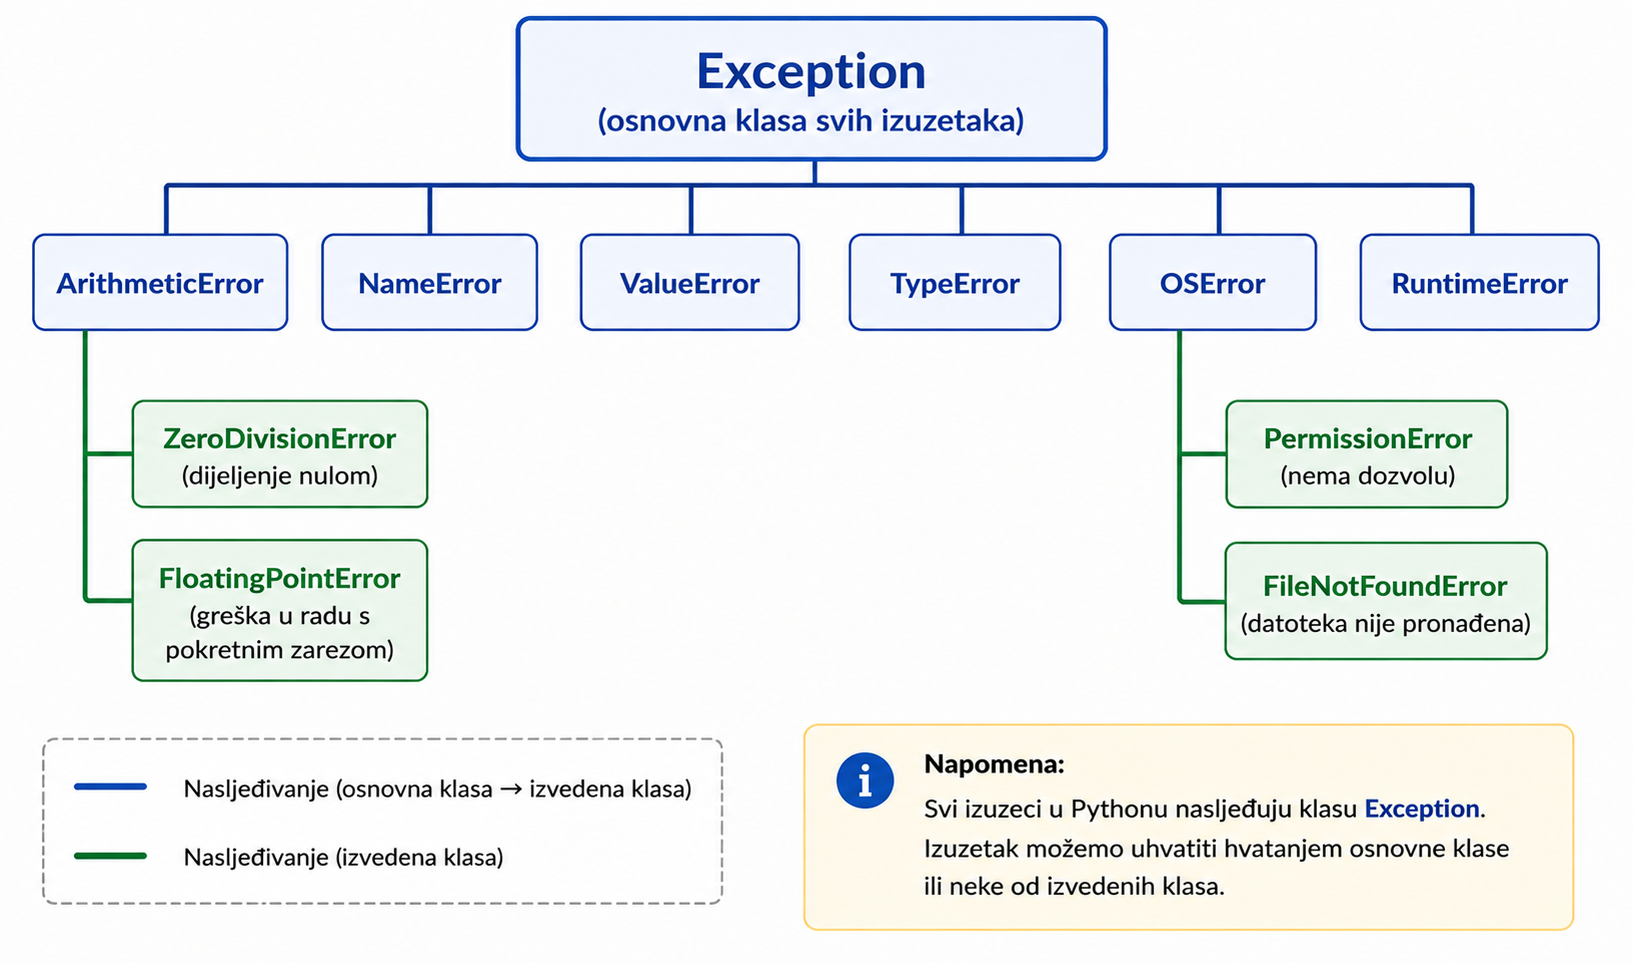
\includegraphics[width=260pt,height=200pt]{slike/class-exceptions.png}
	\caption{Hijerarhija najvažnijih klasa izuzetaka u Pajtonu.}
	\label{fig:exceptions}
\end{figure}

\bigskip

Pravilna upotreba izuzetaka predstavlja važan dio razvoja pouzdanih programa. Obradom izuzetaka moguće je spriječiti neočekivani prekid izvršavanja, korisniku pružiti jasne informacije o nastaloj grešci i povećati robusnost softvera.

\section{Rad sa datotekama}

Pomoću svojih ugrađenih funkcija, Pajton omogućuje jednostavan rad sa ulaznim i izlaznim datotekama. U nastavku dajemo pregled najčešće korište\-nih metoda.

\textit{Čitanje iz datoteke}. Koristimo funkciju \textit{open}(), koja ima dva argu\-menta -- naziv datoteke (ili putanja do datoteke) i način u kojem se otvara datoteka (npr. za čitanje, pisanje, dodavanje, itd.). Pogledajmo sljedeći primjer: 
\begin{minted}{python}
# Otvaranje fajla za citanje
file = open("datoteka.txt", "r")
# Citanje sadrzaja iz fajla 
sadrzaj = file.read()
# Zatvaranje fajla
file.close()
# Ispisivanje sadrzaja fajla 
print(sadrzaj)
\end{minted}

Dakle, prvo otvaramo datoteku  \texttt{datoteka.txt} samo za čitanje. Zatim čitamo sadržaj datoteke koristeći metodu \textit{read}() i čuvamo ga u varijabli \textit{sadrzaj}. Konačno, zatvaramo datoteku pomoću metode \textit{close}() i ispisujemo sadržaj datoteke. 



\textit{Pisanje u fajl}. Za pisanje u datoteku koristimo funkciju \textit{open}(), koja otvara fajl sa određenim nazivom, ali ovaj put sa načinom ``\textit{w}" (eng. \textit{write}), čime se dopušta pisanje u fajl. Pogledajmo sljedeći primjer.
\begin{minted}{python}
# Otvaranje fajla za pisanje
file = open("datoteka.txt", "w")
# Pisanje teksta u datoteku
file.write("Zdravo!")
#  Zatvaranje fajla 
file.close()
\end{minted}


\textit{Dodavanje u fajl}. Da biste dodali sadržaj u postojeći sadržaj datoteke, otvaramo fajl sa načinom ``\textit{a}" (eng. \textit{append}), a potom pomoću funkcije \textit{write}() upisujemo novi sadržaj na postojeći. 

Napomenimo da je dobra praksa zatvoriti datoteku nakon što zavr\-šite rad sa njom, kako bismo izbjegli bilo kakve potencijalne probleme sa oštećenjem datoteke ili gubitkom podataka. Praksa je da se rad u fajlovima odvija pod \textit{try}-\textit{except} blokom. Klase izuzetaka koje se u tim slučajevima mogu koristiti su: \texttt{FileNotFoundError} i \texttt{OSError}. 

% Upis json, csv, ispis itd. 

\subsection{Modul Json}

Modul \texttt{json} se koristi  za enkodiranje i dekodiranje podataka sa i u JSON format (eng. \textit{Java Script Object Notation}) formatu. JSON je  široko raspro\-stranjen format za razmjenu podataka, ljudima jednostavan za čitanje i pisanje, a mašinama za raščlanjivanje i generisanje.\\

Modul \texttt{json} nudi dvije glavne metode za rad sa JSON podacima:


\begin{itemize}
	\item json.\textit{dump}() -- koristi se za enkodiranje pajton objekata u JSON format i njegovo spremanje u objekat  datoteka.
	\item json.\textit{loads}() -- koristi se za dekodiranje JSON niza u pajtonov objekat (obično heš mapa).
\end{itemize}

Pogledajmo i jedan primjer upotrebe \texttt{json} modula. 

\begin{minted}{python}
	import json
	
	# Pajton objekat
	objekat = {'ime': 'Mirko', 'godine': 30, 'grad': 'Banja Luka'}
	# Enkoduj objekat u JSON string
	json_string = json.dumps(objekat)
	# Dekodiraj JSON string nazad u pajtonov objekat (dict)
	dekodiran_objekat = json.loads(json_string)
	
	print(type(json_string))   # <class 'str'>
	print(type(dekodiran_objekat))   # <class 'dict'>
	print(dekodiran_objekat)    # {'ime': 'Mirko', 'godine': 30,
		                        # 'grad': 'Banja Luka'}
\end{minted}


Primijetite da funkcija \textit{dumps}() pretvara pajtonov objekat u string (kodiranje), dok funkcija \textit{loads}() radi obrnutu akciju, od stringa pravi pajtonov objekat (enkodiranje). 

\section{Regularni izrazi}

Regularni izraz (engl. \textit{regular expression}, skraćeno \textit{regex}) predstavlja šablon za opisivanje i pretraživanje tekstualnih nizova. Drugim riječima, regularni izraz definiše skup stringova koji zadovoljavaju određena sintaksna pravila.

Osnovna svrha regularnih izraza jeste da se veliki skup stringova opiše na koncizan način, bez potrebe za njihovim pojedinačnim nabrajanjem. Na primjer, regularnim izrazom možemo opisati skup svih binarnih nizova ili skup riječi {\texttt{gray}, \texttt{grey}} koristeći samo jedan obrazac.

Regularni izrazi imaju široku primjenu u obradi teksta, pretraživanju podataka, validaciji korisničkog unosa, uređivačima teksta i alatima kao što je \texttt{grep} u operativnom sistemu Unix.

\subsection*{Osnovni koncepti regularnih izraza}

\begin{itemize}
	
	\item \textbf{Alternacija}
	
	Alternacija se označava simbolom \texttt{|} i predstavlja logičko ``ili''.
	
	Na primjer, 	$a|b|c $ opisuje skup stringova  $
	\{a,b,c\}.$
	
	\item \textbf{Grupisanje}
	
	Zagrade služe za grupisanje dijelova izraza i određivanje područja djelovanja operatora.
	
	Na primjer, $\texttt{gr}(a|e)\texttt{y}$ opisuje riječi $
	{\texttt{gray},\texttt{grey}}.
	$
	
	\item \textbf{Specijalni simboli i klase karaktera}
	
	\begin{itemize}
		
		\item \texttt{.} -- odgovara proizvoljnom karakteru;
		
		\item \texttt{[abc]} -- odgovara jednom od navedenih karaktera;
		
		\item \texttt{[a-z]} -- odgovara jednom malom slovu engleske abecede;
		
		\item \texttt{[A-Z]} -- odgovara jednom velikom slovu;
		
		\item \texttt{[a-zA-Z]} -- odgovara jednom slovu, bez obzira na veličinu;
		
		\item \texttt{\textbackslash d} -- odgovara jednoj cifri (ekvivalentno izrazu \texttt{[0-9]});
		
		\item \texttt{[\^{}abc]} -- odgovara bilo kojem karakteru osim navedenih;
		
		\item \texttt{\textbackslash w} -- odgovara slovu, cifri ili znaku \texttt{\_};
		
		\item \texttt{\textbackslash s} -- odgovara praznom znaku (razmak, tabulator, novi red);
		
		\item \texttt{\textbackslash n} -- odgovara znaku novog reda;
		
		\item \texttt{\textbackslash t} -- odgovara tabulatoru;
		
		\item \texttt{\textbackslash b} -- odgovara granici riječi.
		
	\end{itemize}
	
	\item \textbf{Kvantifikatori}
	
	Kvantifikatori određuju koliko puta se može pojaviti izraz koji im neposredno prethodi.
	
	\begin{itemize}
		
		\item \texttt{?} -- prethodni izraz pojavljuje se 0 ili 1 put;
		
		\item \texttt{*} -- prethodni izraz pojavljuje se 0 ili više puta;
		
		\item \texttt{+} -- prethodni izraz pojavljuje se 1 ili više puta;
		
		\item \texttt{{m,n}} -- prethodni izraz pojavljuje se najmanje $m$, a najviše $n$ puta.
		
	\end{itemize}
	
\end{itemize}

\subsection*{Primjeri}

\paragraph{Registarske tablice}

Pretpostavimo da registarska oznaka ima oblik:$
\texttt{A12-B-345}$

tj. jedno veliko slovo, dvije cifre, povlaku, jedno veliko slovo, novu povlaku i tri cifre.

Odgovarajući regularni izraz je: $
\texttt{[A-Z]\textbackslash d{2}-[A-Z]-\textbackslash d{3}}$

\paragraph{Datum u formatu DD.MM.GGGG.}

Ako se dan i mjesec uvijek zapisuju sa dvije cifre (npr. \texttt{01.02.2025.}), odgovarajući regularni izraz je: $
\texttt{(\textbackslash d{2})\textbackslash.(\textbackslash d{2})\textbackslash.(\textbackslash d{4})\textbackslash.} $

Ovaj izraz opisuje dvije cifre za dan, dvije cifre za mjesec i četiri cifre za godinu, razdvojene tačkama.

\bigskip

Regularni izrazi predstavljaju veoma moćan alat za obradu tekstualnih podataka. Iako njihova sintaksa na prvi pogled može djelovati složeno, pravilnom kombinacijom osnovnih operatora moguće je veoma precizno opisati i prepoznati složene obrasce u tekstu.

\subsection{Modul Re}

Modul \texttt{re} je ugrađeni Pajtonov modul namijenjen radu sa regularnim izrazima. Omogućava definisanje, pretraživanje i obradu tekstualnih obrazaca (\textit{patterna}), pa predstavlja jedan od najvažnijih alata za manipulaciju tekstualnim podacima.

Da bismo koristili funkcionalnosti ovog modula, potrebno ga je prvo uključiti naredbom:

\begin{minted}{python}
	import re
\end{minted}

Neke od najčešće korištenih funkcija modula \texttt{re} su:

\begin{itemize}
	
	\item \texttt{search(pattern, string)}
	
	Pretražuje string \texttt{string} i pronalazi prvo pojavljivanje obrasca \texttt{pattern}. Ukoliko se obrazac pronađe, funkcija vraća objekat podudaranja (\textit{match object}); u suprotnom vraća vrijednost \texttt{None}.
	
	\item \texttt{match(pattern, string)}
	
	Provjerava da li se obrazac \texttt{pattern} nalazi na samom početku stringa. Ako postoji podudaranje, vraća odgovarajući objekat podudaranja.
	
	\item \texttt{sub(pattern, replacement, string)}
	
	Zamjenjuje sva pojavljivanja obrasca \texttt{pattern} u stringu \texttt{string} novim tekstom \texttt{replacement}.
	
	\item \texttt{split(pattern, string)}
	
	Razdvaja string na dijelove koristeći obrazac \texttt{pattern} kao separator i vraća listu dobijenih podstringova.
	
	\item \texttt{findall(pattern, string)}
	
	Pronalazi sva podudaranja obrasca u stringu i vraća ih u obliku liste.
	
\end{itemize}

U nastavku je prikazan jednostavan primjer korištenja funkcije \texttt{search()}.

\begin{minted}{python}
	import re
	
	# Definisanje obrasca
	
	pattern = r'\b\w+'
	
	# Tekst koji pretražujemo
	text = 'Hello, World!'
	# Pretraga
	match = re.search(pattern, text)
	# Ispis prvog pronađenog podudaranja
	print(match.group())
\end{minted}

Izlaz programa je:

\begin{minted}{text}
	Hello
\end{minted}

Posmatrajmo detaljnije regularni izraz

\begin{minted}{python}
	r'\b\w+'
\end{minted}

Njegove komponente imaju sljedeće značenje:

\begin{itemize}
	\item \texttt{\textbackslash b} označava granicu riječi;
	\item \texttt{\textbackslash w} označava slovo, cifru ili znak \texttt{\_};
	\item \texttt{+} označava jedno ili više uzastopnih pojavljivanja prethodnog obrasca.
\end{itemize}

Dakle, izraz \texttt{\textbackslash b\textbackslash w+} odgovara prvoj riječi u tekstu, odnosno prvom nizu uzastopnih alfanumeričkih znakova koji počinje na granici riječi.

Napomenimo da se u primjeru koristi zapis

\begin{minted}{python}
	r'...'
\end{minted}

koji predstavlja tzv. \textit{raw string}. Kod ovakvog zapisa znak \texttt{\textbackslash} se ne tretira kao početak specijalne sekvence, što pojednostavljuje pisanje regularnih izraza i smanjuje mogućnost greške.

\section{Moduli Sys i Getopt}

\subsection*{Pokretanje programa iz komandne linije}

Pajton skripta se može pokrenuti iz terminala naredbom:

\begin{minted}{bash}
	python myscript.py arg1 arg2
\end{minted}

ili, na sistemima gdje je instalirano više verzija Pajtona,

\begin{minted}{bash}
	python3 myscript.py arg1 arg2
\end{minted}

Pri tome je:

\begin{itemize}
	\item \texttt{myscript.py} naziv skripte;
	\item \texttt{arg1}, \texttt{arg2}, \ldots argumenti komandne linije.
\end{itemize}

\subsection*{Modul Sys}

Modul \texttt{sys} omogućava pristup informacijama i funkcijama vezanim za Pajtonov interpreter i izvršno okruženje.

Neki od najčešće korištenih atributa i funkcija ovog modula su:

\begin{itemize}
	
	\item \texttt{sys.argv}
	
	Lista argumenata komandne linije. Element na poziciji \texttt{0} sadrži naziv skripte, dok ostali elementi predstavljaju argumente koje je korisnik proslijedio programu.
	
	\item \texttt{sys.path}
	
	Lista direktorijuma u kojima Pajton traži module za učitavanje.
	
	\item \texttt{sys.exit([kod])}
	
	Prekida izvršavanje programa i vraća izlazni kod operativnom sistemu. Ukoliko se kod ne navede, podrazumijeva se vrijednost 0.
	
	\item \texttt{sys.version}
	
	Vraća informaciju o verziji Pajtonovog interpretera.
	
	\item \texttt{sys.platform}
	
	Vraća oznaku platforme na kojoj se program izvršava.
	
\end{itemize}

Sljedeći primjer prikazuje korištenje atributa \texttt{argv}.

\begin{minted}{python}
	import sys
	
	if len(sys.argv) > 1:
	    print("Argumenti komandne linije su:")
	
	    for arg in sys.argv[1:]:
	        print(arg)
	 
	else:
	    print("Nema proslijeđenih argumenata.")
\end{minted}

Ako program pokrenemo naredbom

\begin{minted}{bash}
	python test.py arg1 arg2
\end{minted}

dobijamo izlaz

\begin{minted}{text}
	Argumenti komandne linije su:
	arg1
	arg2
\end{minted}

\subsection*{Modul Getopt}

Modul \texttt{getopt} služi za parsiranje opcija i argumenata komandne linije. Njegova funkcionalnost slična je istoimenoj funkciji dostupnoj u Unix operativnim sistemima.

Najvažnija funkcija modula je:

\begin{minted}{python}
	getopt.getopt(args, shortopts, longopts)
\end{minted}

gdje su:

\begin{itemize}
	\item \texttt{args} lista argumenata komandne linije;
	\item \texttt{shortopts} string koji definiše kratke opcije;
	\item \texttt{longopts} lista dugih opcija.
\end{itemize}

Funkcija vraća torku:

\begin{itemize}
	\item listu pronađenih parova \texttt{(opcija, vrijednost)};
	\item listu preostalih argumenata.
\end{itemize}

Na primjer, zapis

\begin{minted}{python}
	"hi:o:"
\end{minted}

definiše tri kratke opcije:

\begin{itemize}
	\item \texttt{-h} ne zahtijeva dodatnu vrijednost;
	\item \texttt{-i} zahtijeva vrijednost;
	\item \texttt{-o} zahtijeva vrijednost.
\end{itemize}

Dvotačka nakon oznake opcije označava da opcija mora imati pridruženu vrijednost.

Za duge opcije koristi se lista stringova:

\begin{minted}{python}
	["ifile=", "ofile="]
\end{minted}

Znak \texttt{=} na kraju naziva opcije označava da opcija zahtijeva argument.

\subsubsection*{Primjer}

\begin{minted}{python}
	import getopt
	import sys
	
	def main(argv):
	
	    inputfile = ""
	    outputfile = ""
	
	    try:
	        opts, args = getopt.getopt(
	            argv,
	            "hi:o:", ["ifile=", "ofile="]
	        )
	
	    except getopt.GetoptError:
	        print("test.py -i <inputfile> -o <outputfile>")
	        sys.exit(2)
	
	    for opt, arg in opts:
	
	        if opt == "-h": 
	            print("test.py -i <inputfile> -o <outputfile>")
	            sys.exit()
	
	        elif opt in ("-i", "--ifile"):
	            inputfile = arg
	
	        elif opt in ("-o", "--ofile"):
                outputfile = arg
	
	if __name__ == "__main__":
	main(sys.argv[1:])
\end{minted}

Program se može pokrenuti naredbom

\begin{minted}{bash}
	python3 test.py -i ulaz.txt -o izlaz.txt
\end{minted}

 
U slučaju da korisnik navede neispravne opcije ili izostavi obavezne argumente, aktivira se izuzetak \texttt{GetOptError}, koji se obrađuje u bloku \texttt{try-except}.

\bigskip

\textbf{Napomena.} U savremenim Pajton programima modul \texttt{argparse} uglavnom predstavlja preporučeni način za obradu argumenata komandne linije, jer nudi jednostavniju sintaksu, automatsko generisanje pomoći (\texttt{-h}) i bolju podršku za složenije aplikacije. Modul \texttt{getopt} je i dalje koristan za razumijevanje osnova parsiranja opcija i kompatibilnost sa Unix stilom komandne linije.


\section{Modul NumPy}

\texttt{NumPy} (skraćeno od \textit{Numerical Python}) predstavlja jednu od najvažnijih biblioteka za naučno i numeričko računarstvo u programskom jeziku Pajton. Razvio ju je Travis Oliphant 2005. godine, a značajan dio implementacije napisan je u jezicima \textit{C} i \textit{C++}.

Osnovna struktura podataka biblioteke NumPy je višedimenzionalni niz (\texttt{ndarray}), koji omogućava efikasan rad sa vektorima, matricama i višedimenzionalnim tenzorima.

Za razliku od Pajtonovih lista:

\begin{itemize}
	\item svi elementi NumPy niza moraju biti istog tipa;
	\item podaci se čuvaju u neprekidnom bloku memorije;
	\item aritmetičke operacije nad nizovima izvršavaju se veoma efikasno;
	\item zauzeće memorije je manje nego kod odgovarajućih lista.
\end{itemize}

Zbog toga su NumPy nizovi posebno pogodni za obradu velikih količina numeričkih podataka.

\begin{figure}[H]
	\centering
	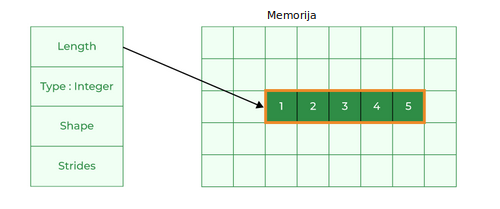
\includegraphics[width=280pt,height=140pt]{slike/numpy-array-memory.png}
	\caption{Pojednostavljen prikaz memorijske organizacije NumPy niza.}
	\label{fig:numpy_array}
\end{figure}

\subsection*{Kreiranje NumPy nizova}

Biblioteka se najčešće uključuje sljedećom naredbom:

\begin{minted}{python}
	import numpy as np
\end{minted}

Primjeri kreiranja jednodimenzionalnih i višedimenzionalnih nizova:

\begin{minted}{python}
	import numpy as np
	
	# Jednodimenzionalni niz
	
	arr = np.array([2, 4, 1, 10], dtype=np.int32)
	
	# Matrica (2D niz)
	
	matrica = np.array(
	[[2, 5],
	[1, 7]],
	dtype=np.int32
	)
	
	# Trodimenzionalni niz
	
	matrica3D = np.array(
	[
	[[2, 5], [1, 7]],
	[[2, 3], [5, 5]]
	],
	dtype=np.int32
	)
\end{minted}

Argument \texttt{dtype} određuje tip podataka koji se koristi za skladištenje elemenata. Neki od najčešćih tipova su:

\begin{center}
	\begin{tabular}{ll}
		\textbf{Tip} & \textbf{Značenje} \\ \hline
		\texttt{int32}, \texttt{int64} & cijeli brojevi \\
		\texttt{float32}, \texttt{float64} & realni brojevi \\
		\texttt{bool} & logičke vrijednosti \\
		\texttt{complex128} & kompleksni brojevi \\
		\texttt{str} & stringovi  \\ \hline \hline
	\end{tabular} 
\end{center}

\subsection*{Osnovne operacije}

\begin{itemize}
	
	\item \textbf{Pristup elementima}
	
	\begin{minted}{python}
		arr[2]           # element 1D niza
		matrica[1, 0]   # element matrice
	\end{minted}
	
	\item \textbf{Dimenzije niza}
	
	\begin{minted}{python}
		arr.shape
	\end{minted}
	
	Atribut \texttt{shape} vraća dimenzije niza.
	
	\item \textbf{Rezanje (slicing)}
	
	\begin{minted}{python}
		arr[1:5]
		arr[::2]
	\end{minted}
	
	\item \textbf{Kopiranje}
	
	\begin{minted}{python}
		kopija = arr.copy()
	\end{minted}
	
	\item \textbf{Promjena oblika}
	
	\begin{minted}{python}
		arr.reshape((2, 2))
	\end{minted}
	
	Broj elemenata mora ostati nepromijenjen.
	
	\item \textbf{Spajanje nizova}
	
	\begin{minted}{python}
		np.concatenate((arr1, arr2), axis=0)
	\end{minted}
	
	\item \textbf{Dijeljenje niza}
	
	\begin{minted}{python}
		np.array_split(arr, 3)
	\end{minted}
	
	\item \textbf{Pretraga elemenata}
	
	\begin{minted}{python}
		np.where(arr % 2 == 0)
	\end{minted}
	
	Vraća indekse elemenata koji zadovoljavaju dati uslov.
	
	\item \textbf{Sortiranje}
	
	\begin{minted}{python}
		np.sort(arr)
	\end{minted}
	
	\item \textbf{Filtriranje}
	
	\begin{minted}{python}
		arr = np.array([41, 42, 43, 44])
		
		filter_arr = arr > 42
		novi_arr = arr[filter_arr]
	\end{minted}
	
	Rezultat je niz:
	
	\begin{minted}{python}
		array([43, 44])
	\end{minted}
	
	\item \textbf{Kreiranje specijalnih nizova}
	
	\begin{minted}{python}
		np.zeros((3, 4))
		np.ones((2, 5))
	\end{minted}
	
\end{itemize}

\subsection*{Vektorizovane operacije}

Jedna od najvećih prednosti biblioteke NumPy jeste mogućnost izvođenja operacija nad cijelim nizovima bez eksplicitnog korištenja petlji.

\begin{minted}{python}
	a = np.array([1, 2, 3])
	b = np.array([4, 5, 6])
	
	c = a + b
\end{minted}

Rezultat je

\begin{minted}{python}
	array([5, 7, 9])
\end{minted}

Na isti način moguće je izvršavati množenje, dijeljenje, poređenja i brojne matematičke operacije nad kompletnim nizovima.

\subsection*{Memorijska organizacija}

Objekti biblioteke NumPy implementirani su klasom \texttt{ndarray}. Pored samih podataka, svaki objekat sadrži i određene metapodatke:

\begin{itemize}
	\item \texttt{dtype} -- tip elemenata niza;
	\item \texttt{ndim} -- broj dimenzija;
	\item \texttt{shape} -- dimenzije niza;
	\item \texttt{strides} -- broj bajtova koji je potrebno preskočiti da bi se došlo do sljedećeg elementa u određenoj dimenziji;
	\item \texttt{data} -- pokazivač na memorijsku oblast u kojoj se nalaze elementi niza.
\end{itemize}

Pošto su elementi smješteni u neprekidnom bloku memorije i imaju isti tip, pristup podacima i izvođenje numeričkih operacija znatno su efikasniji nego kod standardnih Pajtonovih lista.

\section{Modul Ctypes}

Modul \texttt{ctypes} omogućava pozivanje funkcija i korištenje tipova podataka definisanih u dijeljenim bibliotekama (\textit{shared libraries}) napisanim u jeziku \textit{C} ili drugim jezicima nižeg nivoa. Na taj način moguće je koristiti postojeći kôd napisan u jeziku \textit{C} direktno iz Pajtona, bez potrebe za ponovnom implementacijom.

Osnovni koraci za korištenje modula \texttt{ctypes} su sljedeći:

\begin{enumerate}
	\item Napisati program ili biblioteku u jeziku \textit{C}.

	\item Prevesti (\textit{kompajlirati}) program u dijeljenu biblioteku.
	
	Na Linux i macOS sistemima to se obično radi pomoću kompajlera \texttt{gcc}, dok se na Windows sistemima mogu koristiti Visual Studio ili MinGW.
	
	\item Učitati biblioteku u Pajton pomoću modula \texttt{ctypes}.
	
	\item Definisati tipove argumenata i povratne tipove funkcija koje želimo pozivati.
	
	\item Pozvati funkcije iz Pajtona kao da su obične Pajtonove funkcije.
\end{enumerate}

\subsection*{Primjer korištenja}

Pretpostavimo da želimo koristiti jednostavnu funkciju za sabiranje napisanu u jeziku \textit{C}.

\begin{minted}{C}
	// datoteka dodaj.c
	
	int saberi(int a, int b)
	{
		return a + b;
	}
\end{minted}

Na Linux sistemu biblioteku možemo kompajlirati naredbom:

\begin{minted}{bash}
	gcc -shared -fPIC -o libdodaj.so dodaj.c
\end{minted}

Nakon toga biblioteku učitavamo u Pajton:

\begin{minted}{python}
	import ctypes
	
	lib_dodaj = ctypes.CDLL("./libdodaj.so")
\end{minted}

Potom definišemo tipove argumenata i povratni tip funkcije:

\begin{minted}{python}
	saberi = lib_dodaj.saberi
	
	saberi.argtypes = [ctypes.c_int, ctypes.c_int]
	saberi.restype = ctypes.c_int
\end{minted}

Konačno, funkciju možemo pozvati na uobičajen način:

\begin{minted}{python}
	rezultat = saberi(2, 3)
	
	print(rezultat)   # Output: 5
\end{minted}

Modul \texttt{ctypes} automatski vrši konverziju između Pajtonovih i \textit{C} tipova podataka, što značajno pojednostavljuje komunikaciju između ova dva jezika.

\section{Pisanje prilagođenih modula}

Jedna od prednosti programskog jezika Pajton jeste mogućnost organizovanja koda u module. Modul predstavlja datoteku sa ekstenzijom \texttt{.py} koja sadrži funkcije, klase, konstante ili druge definicije koje se mogu koristiti u više programa.

Na primjer, pretpostavimo da želimo napraviti modul za osnovne matematičke operacije. Kreirajmo datoteku \texttt{mathOps.py} sa sljedećim sadržajem:

\begin{minted}{python}
	def add(x, y):
	    return x + y
	
	def subtract(x, y):
	    return x - y
	
	def multiply(x, y):
	    return x * y
	
	def divide(x, y):
	    if y == 0:
	        raise ValueError("Dijeljenje nulom nije dozvoljeno.")
	    return x / y
\end{minted}

Ovaj modul definiše četiri funkcije:

\begin{itemize}
	\item \texttt{add()} -- sabiranje dva broja;
	\item \texttt{subtract()} -- oduzimanje dva broja;
	\item \texttt{multiply()} -- množenje dva broja;
	\item \texttt{divide()} -- dijeljenje dva broja.
\end{itemize}

Nakon što je modul sačuvan, može se koristiti u drugoj Pajton skripti pomoću naredbe \texttt{import}:

\begin{minted}{python}
	import mathOps
	
	print(mathOps.add(3, 4))
	# Output: 7
	print(mathOps.divide(10, 2))
	# Output: 5.0
	
\end{minted}

Ako pokušamo izvršiti dijeljenje nulom:

\begin{minted}{python}
	mathOps.divide(10, 0)
\end{minted}

aktiviraće se izuzetak:

\begin{minted}{python}
	ValueError: Dijeljenje nulom nije dozvoljeno.
\end{minted}

Korištenje modula omogućava bolju organizaciju programa, veću ponovnu upotrebljivost koda i jednostavnije održavanje većih projekata. U praksi se složeni programi gotovo uvijek organizuju kao skup međusobno povezanih modula.

\section{Postavljanje korisnički kreiranih modula na PyPI repozitorij}

PyPI (\textit{Python Package Index}) predstavlja centralni repozitorijum paketa napisanih u programskom jeziku Pajton. Objavljivanjem paketa na PyPI-u omogućava se njegovo jednostavno distribuiranje i instaliranje od strane drugih korisnika.

Da bismo objavili vlastiti paket na PyPI-u, potrebno je izvršiti nekoliko koraka.

Prije svega, potrebno je kreirati korisnički nalog na zvaničnoj PyPI stranici:

\begin{center}
	\texttt{https://pypi.org/account/register/}
\end{center}

Nakon registracije preporučuje se kreiranje API tokena koji služi za sigurnu autentifikaciju prilikom postavljanja paketa na PyPI.

\subsection*{Priprema paketa}

Pretpostavimo da imamo paket pod nazivom \texttt{modul1}. U korijenskom direktorijumu projekta kreiramo datoteku \texttt{pyproject.toml} koja sadrži osnovne metapodatke o paketu:

\begin{minted}{toml}
	[build-system]
	requires = ["setuptools>=61.0"]
	build-backend = "setuptools.build_meta"
	
	[project]
	name = "modul1"
	version = "0.0.1"
	authors = [
	{name = "Mirko Mirković"}
	]
	description = "Primjer korisničkog modula"
	dependencies = [
	"numpy",
	"pandas"
	]
\end{minted}

Ova datoteka definiše naziv paketa, verziju, autora, opis i zavisnosti koje će biti automatski instalirane zajedno sa paketom.

\subsection*{Instalacija potrebnih alata}

Za izgradnju i objavljivanje paketa potrebno je instalirati nekoliko pomoćnih alata:

\begin{minted}{bash}
	pip install build twine
\end{minted}

Paket \texttt{build} služi za kreiranje distribucionih datoteka, dok \texttt{twine} omogućava njihovo postavljanje na PyPI.

\subsection*{Kreiranje distribucije}

Distribucione datoteke kreiraju se naredbom:

\begin{minted}{bash}
	python -m build
\end{minted}

Nakon uspješnog izvršavanja ove naredbe kreira se direktorijum \texttt{dist} koji sadrži:

\begin{itemize}
	\item izvornu distribuciju (\texttt{.tar.gz});
	\item binarnu distribuciju (\texttt{.whl}).
\end{itemize}

\subsection*{Objavljivanje paketa}

Prije objavljivanja preporučuje se provjera ispravnosti generisanih datoteka:

\begin{minted}{bash}
	twine check dist/*
\end{minted}

Paket se zatim objavljuje naredbom:

\begin{minted}{bash}
	twine upload dist/*
\end{minted}

Prilikom objavljivanja koristi se korisničko ime \texttt{\_\_token\_\_} i prethodno generisani PyPI API token.

Nakon uspješnog postavljanja paket postaje dostupan svim korisnicima putem PyPI repozitorijuma.

\subsection*{Instalacija objavljenog paketa}

Objavljeni paket može se instalirati standardnom \texttt{pip} naredbom:

\begin{minted}{bash}
	pip install modul1
\end{minted}

Nakon instalacije paket se može koristiti u bilo kojem Pajton programu:

\begin{minted}{python}
	import modul1
\end{minted}

Objavljivanje paketa na PyPI-u predstavlja standardni način distribucije Pajton softvera i omogućava jednostavno dijeljenje biblioteka sa širom programerskom zajednicom.

\section{Kompajliranje i izvršavanje programa}

U ovom odjeljku ukratko opisujemo način na koji se izvršava program napisan u programskom jeziku Pajton, kao i osnovne principe organizacije memorije tokom rada programa.

\subsection{Stek i hip memorija}

Tokom izvršavanja programa operativni sistem i Pajtonov interpreter koriste različite dijelove memorije. Među njima posebno su važni \textit{stek} (\textit{stack}) i \textit{hip} (\textit{heap}).

\textbf{Stek} predstavlja memorijski prostor koji se koristi za čuvanje informacija o aktivnim pozivima funkcija. Svaki put kada se pozove funkcija, na steku se kreira novi zapis (engl. \textit{stack frame}) koji sadrži informacije potrebne za izvršavanje te funkcije.

Kada funkcija završi rad, njen zapis se uklanja sa steka. Zbog toga kažemo da je stek privremena memorijska struktura čiji je životni vijek vezan za trajanje poziva funkcije.

Posmatrajmo sljedeći primjer:

\begin{minted}{python}
	def func():
	    a = 10
	    b = []
	    c = "abc"
\end{minted}

Prilikom poziva funkcije \texttt{func()} kreira se novi zapis na steku. U njemu se čuvaju reference na objekte označene imenima \texttt{a}, \texttt{b} i \texttt{c}. Nakon završetka funkcije ove reference se uklanjaju iz memorije steka.

Međutim, stvarni objekti na koje reference pokazuju uglavnom se nalaze u drugom dijelu memorije koji se naziva \textbf{hip} (\textit{heap}).

Hip predstavlja dinamički dio memorije namijenjen skladištenju objekata čija veličina može biti poznata tek tokom izvršavanja programa. Gotovo svi Pajton objekti, uključujući liste, rječnike, skupove, torke, stringove i numeričke vrijednosti, smještaju se u hip memoriju.

Na primjer:
\begin{minted}{python}
	a = [0] * 10
\end{minted}

U ovom slučaju lista od deset elemenata kreira se u hip memoriji, dok varijabla \texttt{a} predstavlja referencu na taj objekat.

Za razliku od jezika \textit{C} i \textit{C++}, gdje programer često mora ručno upravljati memorijom, u Pajtonu se dodjeljivanje i oslobađanje memorije obavlja automatski. Interpreter vodi računa o tome kada je potrebno kreirati novi objekat i kada se memorija može osloboditi.

\subsection{Sakupljanje otpadaka}

Pajton koristi mehanizam poznat pod nazivom \textit{garbage collection} (sakupljanje otpadaka). Njegov zadatak je automatsko uklanjanje objekata koji više nisu dostupni nijednom dijelu programa.

Osnovni mehanizam zasniva se na brojanju referenci. Svaki objekat vodi evidenciju o broju aktivnih referenci koje pokazuju na njega. Kada broj referenci postane jednak nuli, objekat se može ukloniti iz memorije.

Pored toga, Pajton koristi i dodatni algoritam za otkrivanje kružnih referenci, odnosno situacija u kojima dva ili više objekata međusobno referenciraju jedni na druge, ali više nisu dostupni ostatku programa.

Zahvaljujući ovim mehanizmima, programer u većini slučajeva ne mora voditi računa o ručnom oslobađanju memorije, što značajno pojednostavljuje razvoj softvera i smanjuje mogućnost pojave memorijskih grešaka.

\subsection{Proces prevođenja i izvršavanja programa}

Iako se Pajton često opisuje kao interpretirani programski jezik, proces izvršavanja programa zapravo uključuje i fazu prevođenja izvornog koda. Zbog toga se može reći da je Pajton istovremeno i kompajlirani i interpretirani jezik.

Proces izvršavanja programa sastoji se od nekoliko osnovnih koraka.

\begin{enumerate}
	
	\item \textbf{Leksička analiza}
	
	Izvorni kôd najprije prolazi kroz leksički analizator koji ga razlaže na elementarne cjeline nazvane \textit{tokeni}. Primjeri tokena su ključne riječi, identifikatori, operatori, literali i interpunkcijski simboli.
	
	\item \textbf{Sintaksna analiza}
	
	Dobijeni tokeni prosljeđuju se parseru koji na osnovu gramatičkih pravila jezika gradi \textit{apstraktno sintaksno stablo} (\textit{Abstract Syntax Tree -- AST}). AST predstavlja hijerarhijsku strukturu programa i služi kao osnova za naredne faze prevođenja.
	
	\item \textbf{Generisanje bajtkoda}
	
	Na osnovu AST strukture Pajton generiše \textit{bajtkod} (\textit{bytecode}), koji predstavlja međureprezentaciju nezavisnu od operativnog sistema i procesorske arhitekture.
	
	Generisani bajtkod može biti sačuvan u datotekama sa ekstenzijom \texttt{.pyc}.
	
	\item \textbf{Izvršavanje bajtkoda}
	
	Bajtkod izvršava Pajtonova virtuelna mašina (\textit{Python Virtual Machine -- PVM}). Virtuelna mašina čita instrukcije bajtkoda i izvršava ih jednu po jednu, upravljajući memorijom, objektima i tokom programa.

\end{enumerate}

Pojednostavljen prikaz procesa izvršavanja prikazan je na Slici~\ref{fig:comp_interpreting}.

\begin{figure}[H]
	\centering
	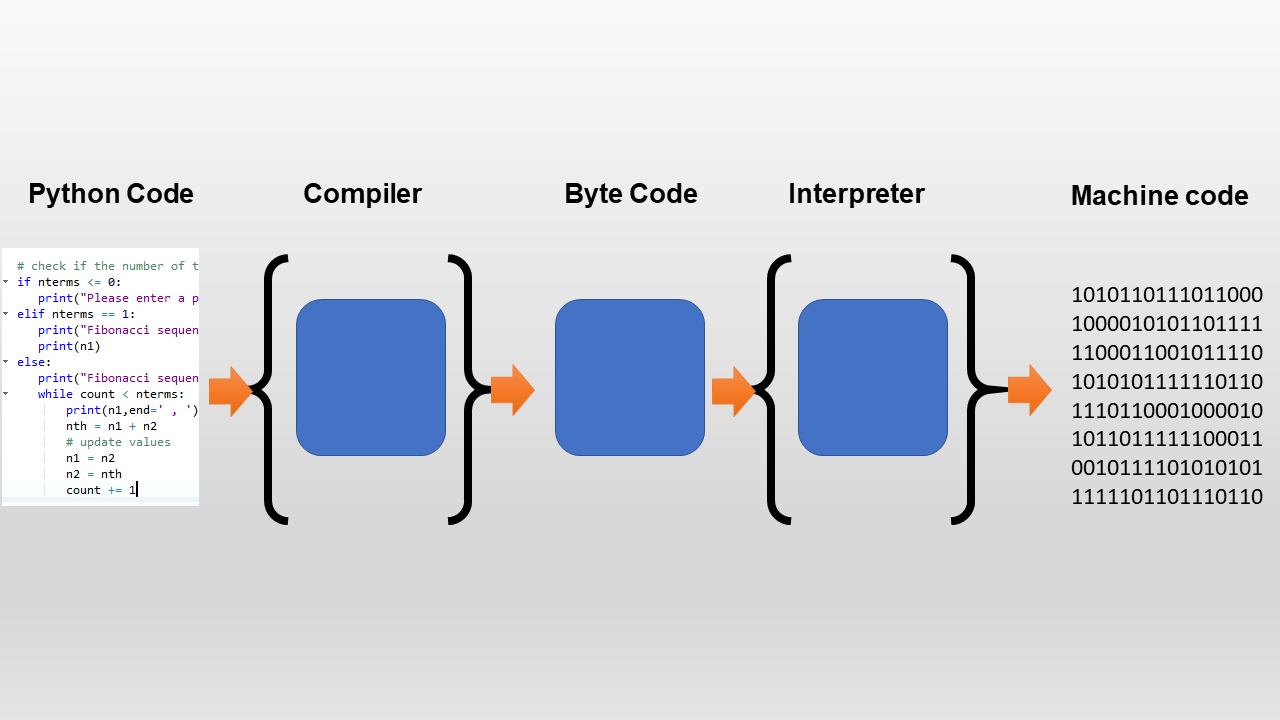
\includegraphics[width=350pt,height=170pt]{slike/python-code-copiler-machine-code.png}
	\caption{Pojednostavljen prikaz procesa prevođenja i izvršavanja Pajton programa.\protect\footnotemark}
	\label{fig:comp_interpreting}
\end{figure}

\footnotetext{Slika preuzeta sa: \texttt{https://www.astateofdata.com/python-programming/can-python-be-compiled/}}

\subsection{Pajtonova virtuelna mašina}

Pajtonova virtuelna mašina (PVM) predstavlja centralnu komponentu izvršnog okruženja jezika Pajton. Njena osnovna uloga jeste izvršavanje bajtkoda generisanog tokom procesa prevođenja izvornog programa.

Najvažnije funkcije PVM-a su:

\begin{itemize}
	
	\item \textbf{Prenosivost programa}
	
	Bajtkod je nezavisan od konkretne hardverske platforme. Zbog toga se isti Pajton program može izvršavati na različitim operativnim sistemima bez izmjene izvornog koda.
	
	\item \textbf{Izvršavanje bajtkoda}
	
	PVM interpretira instrukcije bajtkoda i prevodi ih u odgovarajuće operacije nad objektima i memorijom.
	
	\item \textbf{Dinamičko tipiziranje}
	
	Pošto se tipovi objekata određuju tokom izvršavanja programa, PVM upravlja svim provjerama i operacijama vezanim za tipove podataka.
	
	\item \textbf{Upravljanje memorijom}
	
	PVM koristi mehanizme brojanja referenci i sakupljanja otpadaka (\textit{garbage collection}) kako bi automatski oslobađala memoriju koja više nije potrebna.
	
	\item \textbf{Podrška za module i biblioteke}
	
	PVM omogućava učitavanje i korištenje velikog broja ugrađenih i eksternih biblioteka pomoću naredbe \texttt{import}.

\end{itemize}

Treba napomenuti da standardna implementacija Pajtona (CPython) koristi interpretaciju bajtkoda. Postoje i druge implementacije, kao što su PyPy, Jython i IronPython, koje koriste drugačije tehnike izvršavanja i optimizacije programa.

Na osnovu svega navedenog može se zaključiti da Pajton prvo prevodi izvorni kôd u bajtkod, a zatim taj bajtkod izvršava pomoću virtuelne mašine. Zbog toga se često kaže da je Pajton hibrid između kompajliranih i interpretiranih programskih jezika.


\section*{Zadaci}
%regularni izrazi:
\begin{enumerate}
    %%https://adriann.github.io/programming_problems.html
    
    \item Implementi igru pogađanja u kojoj korisnik treba da pogodi skriveni broj. Nakon pogađanja, program izvještava korisnika da li je njegov broj velik ili mali (ili je pogođen). Na kraju ispisati broj  pokušaja iz kojeg je korisnik pogodio skriveni broj. Računa se jedan pokušaj ukoliko se unese isti broj više puta uzastopno.
    
    
	\item Napisati program koji računa sljedeću sumu  
	
	$$ 4 \cdot \sum_{k=1}^{10^6}(-1)^{k-1} \frac{1}{2k-1}= 4 \cdot (1-1/3 + 1/5-1/7+1/9-1/11 \ldots).$$
	
	\item Napisati funkciju koja kombinira dvije liste naizmjenično uzimajući elemente jedne pa druge liste, Npr. za $[a,b,c], [5, 6, 7]$ generišemo listu $[a,5,b,6,c,7]$.
	
	\item Napisati funkciju koja pomijera elemente liste za $k$ elemenata. Npr. lista  $[1,2,3,4,5,6]$ rotirana za $k=2$ je data sa $[3,4,5,6,1,2]$. Riješiti zadatak bez kreiranja kopije liste. 
	
	\item Napisati funkciju koja uzima broj i vraća listu njegovih brojeva. Npr. za broj $2342$ treba vratiti listu $[2,3,4,2]$.
	
	\item Napisati funkciju koja uzima listu brojeva,   bazu $b_1$ u kojoj se brojevi liste interpretiraju, te ciljnu bazu $b_2$.  Kao rezultat vratiti listu brojeva konvertujući svaki od brojeva početne liste u bazu $b_2$. Npr. za listu $[21,10,01]$ u bazi $b_1 = 3$ pretvaramo u listu brojeva po bazi $b_2=10$, pri čemu vraćamo listu $[7,3, 1]$.
	
	\item Napišite funkciju koja množi dvije matrice. Vratiti grešku (koristiti izuzetke) ukoliko su dimenzije matrica nekompatibilne.  
	 
	\item Napisati regularni izraz koji prepoznaje registarske tablice. Testirati primjenu tog paterna uz pomoć modula \texttt{re}.
	
	\item Napisati regularni izraz koji prepoznaje email adrese. Testirati primjenu tog paterna uz pomoć modula \texttt{re}.
	
	\item Napisati regularni izraz koji prepoznaje realne brojeve (u decimalnom ili eksponencijalnom zapisu). Testirati primjenu uz pomoć modula \texttt{re}.
	
	
	\item Kreirati datoteku \textit{apsolventi}.txt i popuniti je podacima gdje je u svakom redu data
	informacija o studentu apsolventu u formi: 
	 $$<Ime\_prezime>, <datum\_upisa\_na\_fakultet>, <godine\_starosti>$$ 
	
	Datum se zadaje u formi $<$broj$>$.$<$broj$>$.$<$broj$>$. Napisati skriptu koja se pokreće sa terminala čiji su argumenti komandne linije:
	\begin{itemize}
		\item  	\textit{i}: koja zadaje ulaznu datoteku (apsolutna putanja) koja treba da bude učitana u
	program;
	     \item \textit{o}: koja zadaje izlaznu datoteku (apsolutna putanja) u kojoj se čuvaju rezultati	izvršavanja programa;
	     \item  \textit{z}: koji zadaje zadatak koji treba da bude izvršen i obuhvata sljedeći opseg vrijednosti: 
	     \begin{itemize}
	     	\item  1: U izlaznoj datoteci treba da se ispišu svi apsolventi stariji od 25 godina.
             \item 2: U izlaznoj datoteci treba da se ispišu svi apsolventi koji su upisali fakultet u periodu od 01.01.2014.\ do 01.01.2015. godine.
	         \item 3: U izlaznoj datoteci treba da se ispiše sortiran niz (koristiti merge sort) studenata po godini starosti.
	         \item 4: U izlaznoj datoteci treba da se ispiše za svakog studenta koliko godina studira/je studirao.
	        \item Za ostale inpute javiti poruku o neispravnoj opciji (unosu). Koristiti izuzetke.
	         \end{itemize}
       \end{itemize}
	\textit{Napomena}. Studenta učitati uz pomoć regularnih izraza. Dakle, prazan karakter predstavlja 
	invarijantna vrijednost što se postiže konstru\-kcijom odgovarajućeg regularnog izraza koji parsira  sadržaj svakog reda  datoteke.
	
   \item Kreirati datoteku \emph{pretplatnik.txt} i popuniti je podacima gdje je u svakom redu
   data informacija o pretplatniku u formi
   
   $$<Ime\_prezime>, <datum\_ugovora>, <cijena\_usluge>$$
   
   Datum se zadaje u formi $<$broj$>$.$<$broj$>$.$<$broj$>$, a cijena je decimalni broj. Napisati 
   skriptu koja se pokreće sa terminala sa sljedećim argumentima komandne linije:
   \begin{itemize}
   	\item \textit{i}: koja zadaje ulaznu datoteku (apsolutna putanja) koja treba da bude učitana
   u program;
   \item \textit{o}: koja zadaje izlaznu datoteku (apsolutna putanja) koja treba da sačuva
   rezultate izvršavanja programa;
    \item \textit{z}: koji zadaje zadatak koji treba da bude izvršen i obuhvata sljedeće vrijednosti:
    \begin{itemize}
    	\item  1: U izlaznoj datoteci treba da se ispišu svi korisnici koji koriste usluge čija je  cijena veća od 15.4 KM. Elimini\-sati duplikate. 
        \item 2: U izlaznoj datoteci treba da se ispišu svi pretplatnici koji su potpisali ugovor u periodu od 01.01.2022.\ do 15.01.2023. godine.
        \item  3: U izlaznoj datoteci treba da se ispiše zbir svih cijena za usluge koje koristi svaki od pretplatnika. 
        \item 4: U izlaznoj datoteci treba da se ispišu sortirane cijene od najmanje do  najveće.
        \item Za ostale inpute javiti poruku o neispravnoj opciji  (unosu) koristeći izuzetke.
         \end{itemize}
   \end{itemize}
   \textit{Napomena}. Pretplatnika učitati uz pomoć regularnih izraza. Npr., smatra se da je unos Marko
   Markovic, $20.2.2022, 8,4$ isti kao Marko Markovic, $20.\ \ 2.2022, 8,\ \ 4$, itd.  Dakle, prazan karakter predstavlja 
   invarijantnu vrijednost što se postiže konstrukcijom odgovarajućeg regularnog izraza koji parsiraju  sadržaj svakog reda iz datoteke.
\end{enumerate}